\documentclass[pdflatex,sn-mathphys-num]{sn-jnl}
\usepackage[utf8]{inputenc}
\usepackage{textgreek}
\usepackage{tikz}
\usetikzlibrary{positioning,arrows.meta,fit,backgrounds}
\usepackage{amsmath,amssymb,amsfonts}
\usepackage{algorithm}
\usepackage{algpseudocode}
\usepackage{array}
\usepackage{booktabs}
\usepackage{graphicx}
\usepackage{textcomp}
\usepackage{xcolor}
\usepackage{url}
\usepackage{placeins}
\usepackage{hyperref}
\hypersetup{colorlinks=true,linkcolor=black,citecolor=black,urlcolor=black}
\graphicspath{{figures/}}
\raggedbottom
\jyear{2026}

% Change-marking macro. The marked version prints revised text in blue; the clean version prints normal text.
\long\def\rev#1{#1}
% Second-revision changes are printed in blue; replace \color{blue} by \relax for the clean version.
\newcommand{\Rtwo}{\color{blue}}

\begin{document}

\title{\rev{Fed-EITA: Uncertainty- and Trust-Aware Federated Intrusion Detection for Zero-Day IoT Threats}}

\author[1]{Nour A. Kaymih}
\author[1]{Yazan Adnan Mohd Ali}
\author[1]{Haythem A. Bany Salameh}
\affil[1]{Artificial Intelligence Program, College of Engineering, Al Ain University, Al Ain, United Arab Emirates}
\date{}

\maketitle

\begin{abstract}
{\color{black}
The Internet of Things (IoT) connects large numbers of heterogeneous, resource-constrained devices that are frequent targets of cyberattacks, and new attack variants often appear before any labelled examples of them exist. Federated learning (FL) lets these devices train intrusion detectors collaboratively without centralizing their traffic, but federated intrusion detection must cope with two problems that are usually studied separately: attacks that never appear in the training data and clients whose local data are unreliable. Out-of-distribution (OOD) detectors flag unseen inputs but are mostly centralized, whereas robust and trust-aware aggregation limits unreliable clients but does not detect unseen attacks. This paper presents Fed-EITA (Federated Entropy-Informed Trust-Aware intrusion detection), a one-shot, prediction-level federated ensemble of XGBoost clients that couples an uncertainty-based detector of unseen attacks with an interpretable client-trust score. Each client trains one booster on its own traffic and uploads it once, so raw traffic remains local. The server scores every client on a server-held validation split, using the client's validation accuracy and the rate of highly uncertain predictions, and combines the clients' class-probability vectors with the resulting trust weights. Unseen attacks are flagged by fusing normalized entropy, margin-based energy and Mahalanobis scores. The framework is evaluated on TON-IoT in a simulated zero-day setting in which three attack families are withheld from training, and is independently replicated on Edge-IIoT, using training-only preprocessing, Dirichlet non-IID partitions, two label-noisy clients, ten seeds and Holm-corrected paired tests. {\Rtwo At $\alpha_D=0.5$, without being told which clients are noisy, the trust score gives the two label-noisy clients the two lowest weights in 8 of 10 seeds (9 of 10 with three attack families withheld; mean weights 0.151 and 0.172, against 0.225--0.227 for clean clients); this detection rises with the noise rate and is unreliable below 10\% noise. Down-weighting the noisy clients is better than excluding them. Trust weighting reduces the instability of sample-size weighting under moderately non-IID data (98.07\% vs.\ 92.90\% accuracy at $\alpha_D = 0.3$, against 98.16\% for uniform averaging) and attains a zero-day AUROC of 89.39\%, which drops to 85.71\% when test flows that duplicate a training flow are removed.} It does not exceed uniform averaging or coordinate-wise robust aggregation in accuracy, and the fused score is competitive with, but not better than, entropy alone. The complete predictor adds about 16\,ms per 1,000 flows to inference. Code, per-seed results and the table generator are publicly released.}
\end{abstract}

\keywords{\rev{Internet of Things; {\color{black}federated ensemble}; intrusion detection system; federated learning; zero-day attack detection; out-of-distribution detection; uncertainty estimation; trust-aware aggregation. }}

\section{Introduction}
\label{sec:introduction}
The rapid proliferation of Internet of Things (IoT) devices has expanded the cyberattack surface of modern networks \cite{hamad2025systematic,sharma2025leveraging,rahman2025survey,alshdadi2025federated}. These devices generate large volumes of sensitive network traffic \cite{malatji2025artificial,alketbi2025comprehensive} and are increasingly targeted by attacks, including zero-day attacks that are not observed during model training \cite{kim2020ai}. Intrusion detection systems (IDSs) are therefore essential for identifying malicious activity in IoT networks \cite{alsbatin2025enhancing,rahman2020internet}. Traditional signature-based IDSs detect only known attack patterns and remain weak against unknown threats \cite{kim2020ai,alsbatin2025enhancing,rahman2020internet,amrullah2025review,menon2025ai}. Machine learning (ML) and deep learning (DL) models have improved detection on benchmark IoT datasets such as TON-IoT \cite{sharma2025leveraging,alshdadi2025federated,alsbatin2025enhancing,menon2025ai,mohale2025systematic,mallidi2025advancements,hozouri2025comprehensive}; however, many learning-based IDSs still require centralized training on raw traffic, which creates data-governance concerns \cite{hamad2025systematic,alshdadi2025federated}.

Federated learning (FL) allows clients to learn collaboratively without transmitting raw traffic to a central server \cite{rahman2020internet,menon2025ai,al2025privacy,li2020deepfed,ismail2025intrusion}. Most FL-based IDSs aggregate client contributions with Federated Averaging (FedAvg), which weights clients by their sample counts \cite{alshdadi2025federated,menon2025ai,hozouri2025comprehensive}. This weighting is problematic in IoT deployments, because clients differ in traffic distribution and data quality. Highly heterogeneous, non-independent and identically distributed (non-IID) data degrade federated models \cite{zhao2018federated,li2020fedprox,karimireddy2020scaffold}, and clients with unreliable labels contribute unreliable models. A federated IDS should therefore account for both statistical heterogeneity and client reliability.

A second limitation is that most FL-based IDSs are designed for closed-set classification. IoT networks, however, face out-of-distribution (OOD) and zero-day attacks whose traffic patterns are absent from the training data. Uncertainty-based OOD scores, such as entropy, energy, k-nearest-neighbour distances and Mahalanobis distance, can detect distributional shift \cite{liu2020energy,wang2021tent,sun2022knn,lee2018mahalanobis}, but they are usually studied in centralized settings and are not combined with client reliability.  A third limitation concerns how detection outcomes are communicated to analysts. Explainable artificial intelligence (XAI) methods identify influential features \cite{alketbi2025comprehensive,alsbatin2025enhancing,amrullah2025review,menon2025ai,mohale2025systematic,hozouri2025comprehensive}, and recent work has explored lightweight large-language-model-assisted reasoning for IoT security \cite{mohawesh2026lightweight}; uncertainty and client trust, however, are rarely reported alongside the prediction.

{\color{black}
This paper presents Fed-EITA (Federated Entropy-Informed Trust-Aware intrusion detection). Fed-EITA is a one-shot, prediction-level federated ensemble in the sense of one-shot federated learning \cite{guha2019oneshot}: each client trains one XGBoost model and uploads it once, and the server combines the clients' predictions rather than their parameters. The server derives a trust weight for every client from its behaviour on a server-held validation split and fuses three uncertainty scores to flag traffic from unseen attack families. The contributions of this paper are as follows.

\begin{itemize}

\item \textbf{Developing a one-shot federated ensemble for IoT intrusion detection:}
The framework jointly addresses zero-day threats and client reliability. Each client trains and uploads a single XGBoost booster without sharing raw traffic.%, following the protocol detailed in Section~\ref{sec:protocol} and Algorithm~\ref{alg:fedeita}.

\item \textbf{Designing an interpretable, server-side trust score:}
Based on validation accuracy and predictive uncertainty, the score identifies label-noisy clients that accuracy alone fails to distinguish {\Rtwo (in 8--10 of 10 seeds at noise rates of 10\% or more)} % (Table~\ref{tab:trust}) 
and reduces the instability of sample-size weighting under moderately non-IID conditions, %(Table~\ref{tab:agg}), 
without exceeding uniform averaging in accuracy.

\item \textbf{Integrating uncertainty-based OOD detection:}
Entropy, margin-based energy, and Mahalanobis scores derived from aggregatable client statistics are fused to identify unseen attack families.% (Section~\ref{sec:ood}).

\item \textbf{Establishing a leakage-controlled and statistically rigorous evaluation:}
The evaluation includes training-only preprocessing, withheld attack families, family-rotation tests, ten seeds, Holm-corrected paired tests, confidence intervals, effect sizes, robust aggregation comparisons, and independent replication on Edge-IIoT.

\item \textbf{Providing evidence-based insights:}
The results demonstrate that identifying unreliable clients does not necessarily improve accuracy, anomaly-rate-only penalties can harm performance under non-IID conditions, {\Rtwo excluding unreliable clients is worse than down-weighting them, the Mahalanobis term weakens the fused score,} and zero-day detection effectiveness varies across attack families.

\item \textbf{Releasing a reproducible experimental package:}
The released package includes code, configurations, per-seed results, logs, and table-generation scripts to reproduce the reported tables under pinned dependencies, except for measured runtimes.

\end{itemize}

The remainder of the paper is organized as follows. Section~\ref{sec:related_work} reviews related work. Section~\ref{sec:system_model} defines the system model. Section~\ref{sec:framework} presents the framework. Section~\ref{sec:evaluation} describes the experimental protocol and results, and Section~\ref{sec:conclusion} concludes with the limitations of the study.

\section{Related Work}
\label{sec:related_work}

\subsection{Federated Learning for IoT Intrusion Detection}

{\color{black}Federated learning is widely used for IoT intrusion detection because it lets clients learn collaboratively without exposing local traffic \cite{mcmahan2017fedavg,kairouz2021advances,yang2019federated}. FedAvg \cite{mcmahan2017fedavg} remains the most common aggregation strategy. FedProx \cite{li2020fedprox}, SCAFFOLD \cite{karimireddy2020scaffold}, FedNova \cite{wang2020fednova}, model-contrastive federated learning (MOON) \cite{li2021moon} and Ditto \cite{li2021ditto} improve the optimization of a shared parametric model under heterogeneous data. These methods modify gradient-based training and therefore do not apply directly to independently trained boosted trees. Federated gradient-boosting protocols such as SecureBoost \cite{cheng2021secureboost} instead learn a single global booster through repeated exchange of gradient statistics; they are a complementary direction to the one-shot ensemble studied here. Existing FL-based IDSs mainly target classification accuracy rather than zero-day detection or client reliability \cite{javeed2024zerotrust}.}

\subsection{OOD and Zero-Day Attack Detection}
Detecting unseen attacks is difficult because most IDS models are trained under a closed-set assumption. OOD detection estimates whether a test sample deviates from the training distribution \cite{geng2021openset,yang2024oodsurvey}. Energy-based detection separates in-distribution and anomalous samples using the log-sum-exp of the logits \cite{liu2020energy}. Test-time entropy minimization (TENT) adapts model parameters during testing \cite{wang2021tent}. KNN-OOD \cite{sun2022knn} and Mahalanobis-distance detection \cite{lee2018mahalanobis} measure distances from known feature distributions. However, extending these methods to federated intrusion detection introduces additional challenges related to data heterogeneity and client reliability.
{\color{black}
\subsection{Trust-Aware and Robust Federated Learning}
Byzantine-robust aggregation rules such as Krum \cite{blanchard2017machine}, the coordinate-wise median and trimmed mean \cite{yin2018byzantine}, and Bulyan \cite{mhamdi2018hidden} limit the influence of outlying client updates. DeepSight \cite{rieger2022deepsight} instead inspects the structure of model updates to filter backdoored models. Surveys of federated learning for IoT identify unreliable and malicious clients as a central open problem \cite{nguyen2021federated}. FLTrust \cite{cao2021fltrust} is the mechanism closest to ours: the server holds a small root dataset and weights client updates by their agreement in direction with an update computed on that dataset. Fed-EITA also relies on server-held reference data, but derives trust from the accuracy and predictive uncertainty of each client's model on that data rather than from update direction. Federated misbehaviour detection has also been applied to vehicular networks \cite{vinita2023federated}. Zero-trust architectures for IoT continuously verify devices and their access \cite{ijbas2025zerotrust}, and Zero-Trust Agentic Federated Learning (ZTA-FL) \cite{singh2025ztafl} combines trust evaluation, authentication and secure aggregation for industrial IoT. These approaches verify identities and updates; Fed-EITA's trust is a model-level reliability signal and enforces nothing. {\Rtwo Fed-EITA's trust also differs from weighting ensemble members by their validation performance: such weighting corresponds to the accuracy-only variant of our ablation, which gives the label-noisy clients essentially uniform weight (0.202 against 0.200), because their models are as accurate on the reference set as the clean ones; it is the anomaly rate, the share of reference flows on which a client model is highly uncertain, that separates them (Section~\ref{sec:trust_results}). Unlike uncertainty-aware aggregation of parameter updates, the uncertainty is measured on the client model's predictions for common reference data, not on its updates.} None of these methods couples client trust with the detection of unseen attacks.}
\subsection{Comparison with Existing Literature}
Table~\ref{tab:literature} positions Fed-EITA with respect to representative approaches. 

\begin{table}[!htbp]\centering
\color{black}
\caption{Design scope of Fed-EITA and representative federated, robust-aggregation and OOD detection approaches.}\label{tab:literature}
\footnotesize
\begin{tabular}{@{}>{\raggedright\arraybackslash}p{0.27\textwidth}>{\raggedright\arraybackslash}p{0.14\textwidth}>{\raggedright\arraybackslash}p{0.13\textwidth}>{\raggedright\arraybackslash}p{0.20\textwidth}>{\raggedright\arraybackslash}p{0.10\textwidth}@{}}\toprule
Method & Federated & OOD / zero-day detection & Client trust or robustness & Tree-based clients \\ \midrule
FedAvg \cite{mcmahan2017fedavg} & Yes & No & No & No \\
FedProx \cite{li2020fedprox}, MOON \cite{li2021moon} & Yes & No & No & No \\
Krum, Trimmed mean \cite{blanchard2017machine,yin2018byzantine} & Yes & No & Robust aggregation & No \\
FLTrust \cite{cao2021fltrust} & Yes & No & Server root-data trust & No \\
SecureBoost \cite{cheng2021secureboost} & Yes & No & No & Yes \\
Energy-OOD \cite{liu2020energy}, KNN-OOD \cite{sun2022knn} & No & Yes & No & No \\
ZTA-FL \cite{singh2025ztafl} & Yes & No & Trust and authentication & No \\
\textbf{Fed-EITA (ours)} & \textbf{Yes (one-shot ensemble)} & \textbf{Yes (simulated)} & \textbf{Server-side reliability score} & \textbf{Yes} \\
\bottomrule\end{tabular}
\end{table}
As shown in Table~\ref{tab:literature}, conventional federated learning methods primarily address collaborative model training, while robust aggregation approaches focus on limiting unreliable client contributions. In contrast, standalone OOD detectors target unseen inputs without incorporating federated client reliability. Fed-EITA brings these complementary capabilities together through a one-shot, tree-based federated ensemble that combines server-side client reliability assessment with simulated zero-day detection. This comparison highlights the framework's integration of these capabilities rather than claiming superiority over the individual methods.
%\rev{Table~\ref{tab:literature} highlights the key distinction of Fed-EITA. Existing federated learning methods mainly focus on privacy-preserving distributed optimization, while OOD detection approaches target unseen attack identification in centralized settings. Recent trust-aware frameworks such as ZTA-FL improve aggregation robustness and resistance to unreliable clients but do not explicitly address OOD or zero-day attack detection. In contrast, Fed-EITA jointly integrates federated learning, uncertainty-aware OOD detection, trust-aware aggregation, robustness under Non-IID environments, and noisy-client resistance within a unified intrusion detection framework.}

\FloatBarrier
{\color{black}
\subsection{Research Gap}
Existing methods address only part of the problem. FL algorithms improve distributed training but neglect unseen attacks and unreliable clients. OOD methods detect distributional shift but are usually centralized. Trust-aware and robust FL methods limit unreliable contributions but do not detect zero-day attacks. Table~\ref{tab:gap} summarizes these requirements.}

\begin{table}[!htbp]\centering
\color{black}
\caption{Requirements addressed by federated IDSs, OOD detection methods and Fed-EITA.}\label{tab:gap}
\footnotesize
\begin{tabular}{lccc}\toprule
Requirement & FL-IDS & OOD detection & Fed-EITA \\ \midrule
Raw traffic remains local & \checkmark & $\times$ & \checkmark \\
Detection of unseen (held-out) attack families & $\times$ & \checkmark & \checkmark \\
Client-level reliability assessment & $\times$ & $\times$ & \checkmark \\
Stable aggregation under non-IID partitions & Partial & $\times$ & \checkmark \\
Joint treatment of unseen attacks and client reliability & $\times$ & $\times$ & \checkmark \\
\bottomrule\end{tabular}
\end{table}
%As summarized in Figure~\ref{fig:research_gap}, there remains a need for a unified framework that jointly supports privacy-preserving FL, uncertainty-aware OOD detection, trust-aware aggregation, non-IID robustness, communication efficiency, and interpretable security reasoning.

%\begin{figure}[htbp!]
%\centering
%\includegraphics[width=0.8\linewidth]{research_gap.png}
%\caption{\rev{Research gap analysis illustrating the limitations of existing FL-based IDS approaches and OOD detection methods. %The figure highlights the absence of a unified framework that jointly addresses federated learning, OOD and zero-day detection, trust-aware aggregation, and robustness under non-IID data distributions.
%}}
%\label{fig:research_gap}
%\end{figure}


\section{System Model and Notation}
\label{sec:system_model}
{\color{black}
We consider a federated IoT environment with $K$ heterogeneous clients and a central server. Each client $i\in\{1,\dots,K\}$ observes local network traffic and holds a private dataset
\begin{equation}
\mathcal{D}_i=\{(\mathbf{x}_{ij},y_{ij})\}_{j=1}^{n_i},\label{eq:data}
\end{equation}
where $\mathbf{x}_{ij}\in\mathbb{R}^d$ is a traffic feature vector, $y_{ij}\in\{1,\dots,C\}$ its class label, $C$ the number of known classes and $n_i$ the number of samples at client $i$. The task is multi-class intrusion classification augmented with an uncertainty score for detecting traffic from unseen attack families.

{\color{black}Because non-IID data are known to degrade federated learning \cite{zhao2018federated}, the training data are partitioned with a class-wise Dirichlet process to simulate them:} for every class $c$, a proportion vector is drawn and the indices of class $c$ are split among the $K$ clients accordingly,
\begin{equation}
\mathbf{q}_c\sim\mathrm{Dir}(\alpha_D\mathbf{1}_K),\qquad |\mathcal{D}_i\cap\mathcal{Y}_c|\approx q_{c,i}\,|\mathcal{Y}_c|,\label{eq:dirichlet}
\end{equation}
where $\mathcal{Y}_c$ is the set of training samples of class $c$ and smaller $\alpha_D$ produces stronger heterogeneity; client $i<K$ receives $n_{c,i}=\lfloor q_{c,i}|\mathcal{Y}_c|\rfloor$ samples of class $c$, and client $K$ receives the remainder $n_{c,K}=|\mathcal{Y}_c|-\sum_{i<K}n_{c,i}$. A client that receives no sample of a class is given a copy of one training sample of that class, drawn at random from the whole training split (the sample also remains with its original client), so that all local models share the same output space. This is a step of the simulated partitioning, performed before local training; in a real deployment it would require sharing one sample per missing class. In the TON-IoT runs, it places at most 12 of the 290{,}457 training rows in two clients. Table~\ref{tab:notation} lists the main symbols.}

\begin{table}[htbp]\scriptsize
\color{black}
\centering
\caption{Main notation.}
\label{tab:notation}
\begin{tabular}{@{}p{0.25\linewidth}p{0.65\linewidth}@{}}
\toprule
\textbf{Symbol} & \textbf{Definition} \\
\midrule

$K$ &
Number of clients ($K=5$) \\

$\mathcal{D}_i,\,n_i$ &
Private training data of client $i$ and its size \\

$\mathcal{V},\,m$ &
Server-held validation (reference) split and its size \\

$d,\,d'$ &
Original and selected feature dimensions ($d'=15$) \\

$C$ &
Number of known classes \\

$f_i$ &
XGBoost booster of client $i$ \\

$\mathbf{P}_i(\mathbf{x}),\,\mathbf{g}_i(\mathbf{x})$ &
Class-probability vector and raw margins of client $i$ \\

$\mathbf{P}_{\mathrm{global}},\,\mathbf{g}$ &
Trust-weighted aggregated probabilities and margins \\

$\boldsymbol{\mu}_c,\,\boldsymbol{\Sigma}_c$ &
Mean and covariance of known class $c$ \\

$a(\mathbf{x}),\,E(\mathbf{x}),\,M(\mathbf{x})$ &
Entropy, energy and Mahalanobis scores; $\tilde a,\tilde E,\tilde M$ after rescaling \\

$T$ &
Energy temperature ($T=1$) \\

$S(\mathbf{x}),\,S_{\mathrm{global}}(\mathbf{x})$ &
Fused uncertainty score; evaluated on the aggregated prediction \\

$\boldsymbol{\beta}$ &
Fusion weights (entropy, energy, Mahalanobis) \\

$z_i(\mathbf{x})$ &
Model-dependent uncertainty of client $i$ (trust only) \\

$\mathrm{Acc}_i$ &
Validation accuracy of client $i$ on $\mathcal{V}$ \\

$\mathrm{AR}_i,\,\tau_{\mathrm{AR}}$ &
Anomaly rate of client $i$ on $\mathcal{V}$ and its threshold \\

$\boldsymbol{\omega}$ &
Trust-signal weights (Eq.~\ref{eq:trust}) \\

$\hat{T}_i^{(r)},\,T_i^{(r)}$ &
Trust estimate and trust memory of client $i$
at trust-update iteration $r$ \\

$R$ &
Number of trust-update iterations ($R=20$) \\

$w_i,\,\mathcal{S}$ &
Normalized aggregation weight of client $i$; set of selected clients \\

$\hat y,\,D(\mathbf{x})$ &
Class prediction and final decision \\

$\Phi,\,\mathrm{Rep}(\mathbf{x})$ &
Rule-based report mapping and its report \\

$\tau_{\mathrm{zd}},\,\tau_T$ &
Zero-day operating threshold and trust threshold \\

$\lambda$ &
Trust-memory factor \\

\bottomrule
\end{tabular}
\end{table}
\section{Proposed Framework: {\color{black} a Prediction-Level Federated Ensemble}}
\label{sec:framework}

\subsection{Threat Model}\label{sec:threat} 

{\color{black}This subsection states exactly what Fed-EITA is designed to withstand and what it is not. The server is honest-but-curious: it follows the protocol and never receives raw traffic, but it may inspect what clients upload. As in FLTrust \cite{cao2021fltrust}, the server is assumed to hold a small labelled validation (reference) set; in our experiments it is a 10\% split of the training data. The study considers unreliable clients whose local labels are corrupted. In the experiments, two of the five clients (40\%) carry symmetric label noise: a fraction of their training labels is replaced by labels drawn uniformly from all classes. Features, predictions and uploaded models are not manipulated, the corruption is present from the start, and clients cannot directly report or modify their trust statistics, because these are computed by the server on its own validation data; they could influence them only indirectly through a manipulated model, which is outside this threat model. In addition, traffic from attack families never seen in training may appear at test time. Adaptive adversaries (model poisoning, backdoors, targeted label flipping, sign flipping and collusion) are outside this threat model. Fed-EITA does not provide formal privacy: raw traffic remains local, but uploaded boosters and per-class statistics may leak information about local data, and neither differential privacy nor secure aggregation is implemented.}
{\color{black}\subsection{Federated Protocol and Exchanged Information}\label{sec:protocol}
Fed-EITA does not train a shared model by iterative averaging: it is a one-shot, prediction-level federated ensemble. This subsection specifies what is computed where and what is transmitted, which determines the communication cost (Section~\ref{sec:cost}) and the privacy scope (Section~\ref{sec:threat}). Algorithm~\ref{alg:fedeita} gives the client and server procedures.
\begin{enumerate}
\item \textbf{Client side (once).} Client $i$ applies the shared preprocessing transform supplied by the protocol (encoding vocabulary, scaling constants and selected features, fitted once on client-training rows only; in our simulation this fit is performed centrally, see Section~\ref{sec:conclusion}), trains an XGBoost booster $f_i$ on its private data and uploads the serialized booster (0.66~MB on TON-IoT). No raw traffic, features or labels leave the client. For the Mahalanobis term, the client also sends per-class counts, sums and second moments of a subsample of its features (Layer 3, Section~\ref{sec:architecture}).
\item \textbf{Server side.} The server evaluates each booster on $\mathcal{V}$ to obtain the validation accuracy $\mathrm{Acc}_i$ and the anomaly rate $\mathrm{AR}_i$ (Eq.~\ref{eq:ar}). It then updates the trust memory (Eqs.~\ref{eq:trust}--\ref{eq:memory}) for $R=20$ iterations on resampled validation mini-batches. These are trust-update iterations, not communication rounds, and they require no additional communication.
\item \textbf{Deployment.} The detector is the trust-weighted ensemble of the $K$ boosters (Eqs.~\ref{eq:weights}--\ref{eq:argmax}), hosted at the server or at an edge gateway. Predicting a new flow never requires sending that flow to the clients.
\end{enumerate}
Because clients are trained once, no model is redistributed, there is no iterative optimization, and the system does not learn a single global model.

{\Rtwo \emph{Server-side assumptions in a deployment.} Three quantities are computed centrally in our simulation. (i) The labelled reference set $\mathcal{V}$ is a 10\% split of the training data, so it follows the training distribution of the known classes. In a deployment it would be traffic that the operator labels itself, for example from a monitored network segment, a honeypot or vetted incident records; it must cover every known class, and the trust score is only as representative as this set (a reference set biased towards some classes favours clients that are strong on those classes). No client traffic is needed for it. (ii) The preprocessing transform: per-feature minima, maxima and category vocabularies can be aggregated from per-client values without sharing flows, whereas the mutual-information ranking would require a federated estimate (for example, aggregated per-client contingency counts of discretized features); this step was not implemented federatively. (iii) The Mahalanobis statistics are sums over clients and can be aggregated exactly (verified to $1.1\times10^{-14}$) and, if required, with secure aggregation. Neither (ii) nor (iii) requires a client to send raw traffic.}

\subsection{Architecture}\label{sec:architecture}
Figure~\ref{fig:architecture} shows the six layers of the framework. Clients preprocess and train once and upload their boosters; the server computes client trust on its validation split, combines client predictions with trust weights and scores each flow for unseen attacks; the outputs are the decision and an optional rule-based report.}


\begin{figure}[!htbp]\centering
{\color{black}
\resizebox{\textwidth}{!}{%
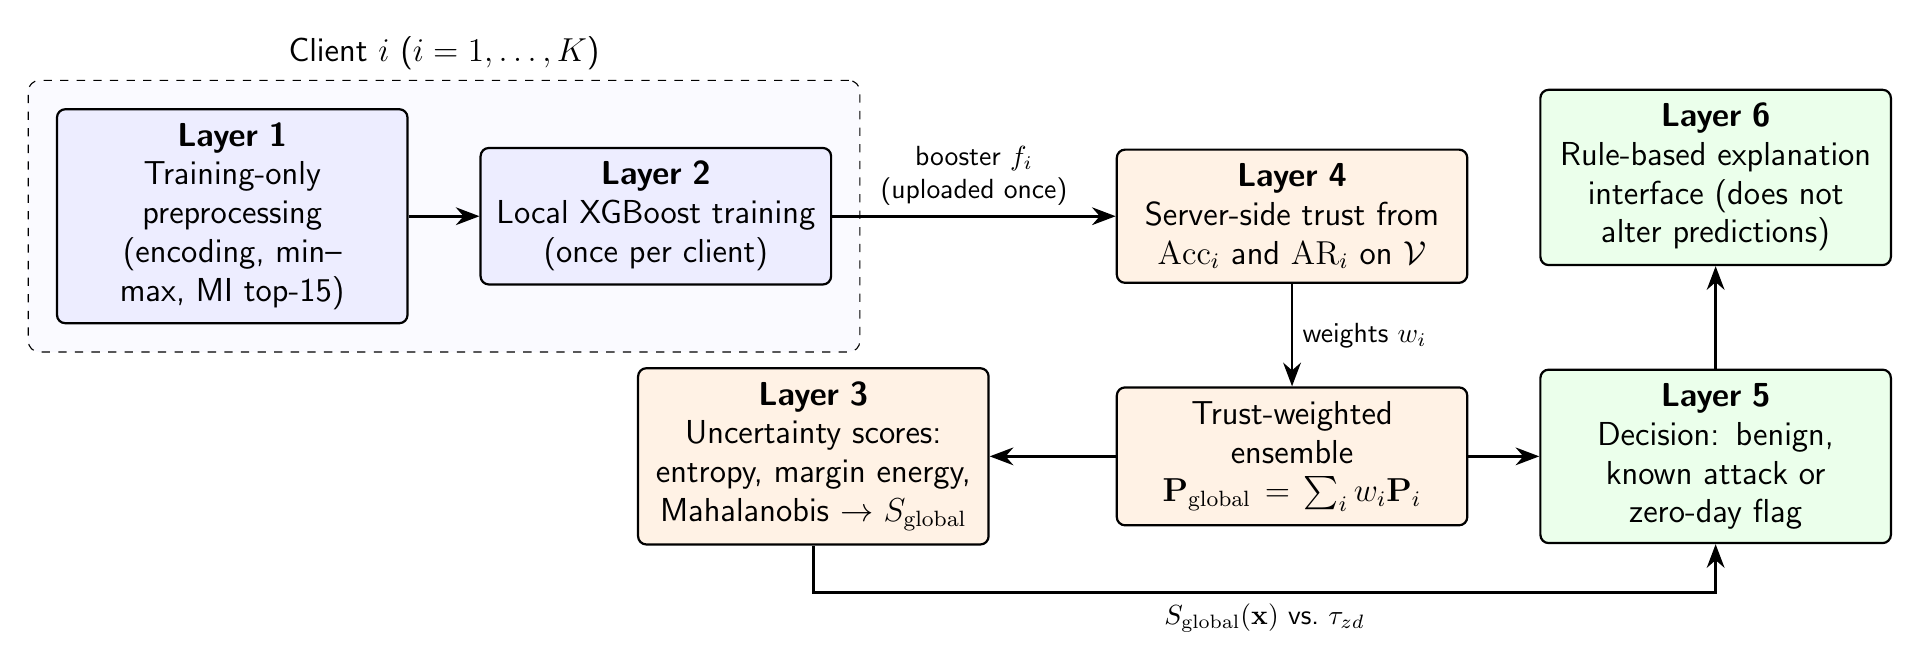
\begin{tikzpicture}[font=\sffamily\large,
  box/.style={draw, rounded corners=3pt, align=center, minimum height=1.55cm, text width=4.1cm, inner sep=5pt, line width=0.8pt},
  cli/.style={box, fill=blue!7}, srv/.style={box, fill=orange!10}, outb/.style={box, fill=green!8},
  arr/.style={-{Stealth[length=3mm]}, line width=1pt}]
\node[cli] (l1) {\textbf{Layer 1}\\Training-only preprocessing\\(encoding, min--max, MI top-15)};
\node[cli, right=0.9cm of l1] (l2) {\textbf{Layer 2}\\Local XGBoost training\\(once per client)};
\node[srv, right=3.6cm of l2] (l4) {\textbf{Layer 4}\\Server-side trust from\\$\mathrm{Acc}_i$ and $\mathrm{AR}_i$ on $\mathcal{V}$};
\node[srv, below=1.3cm of l4] (agg) {Trust-weighted ensemble\\$\mathbf{P}_{\mathrm{global}}=\sum_i w_i\mathbf{P}_i$};
\node[srv, left=1.6cm of agg] (l3) {\textbf{Layer 3}\\Uncertainty scores:\\entropy, margin energy,\\Mahalanobis $\rightarrow S_{\mathrm{global}}$};
\node[outb, right=0.9cm of agg] (l5) {\textbf{Layer 5}\\Decision: benign,\\known attack or\\zero-day flag};
\node[outb, above=1.3cm of l5] (l6) {\textbf{Layer 6}\\Rule-based explanation\\interface (does not\\alter predictions)};
\begin{scope}[on background layer]
\node[draw, dashed, rounded corners, fill=blue!2, fit=(l1)(l2), inner sep=10pt, label={[font=\sffamily\large]above:Client $i$ ($i=1,\dots,K$)}] {};
\end{scope}
\draw[arr] (l1) -- (l2);
\draw[arr] (l2) -- node[above, font=\sffamily\normalsize, align=center]{booster $f_i$\\(uploaded once)} (l4);
\draw[arr] (l4) -- node[right, font=\sffamily\normalsize]{weights $w_i$} (agg);
\draw[arr] (agg) -- (l3);
\draw[arr] (agg) -- (l5);
\draw[arr] (l3.south) -- ++(0,-0.6) -| node[pos=0.25, below, font=\sffamily\normalsize]{$S_{\mathrm{global}}(\mathbf{x})$ vs.\ $\tau_{zd}$} (l5.south);
\draw[arr] (l5) -- (l6);
\end{tikzpicture}}
\caption{Fed-EITA architecture: clients (blue) train once and upload boosters; the server (orange) computes trust, aggregates and scores; outputs are green.}\label{fig:architecture}}
\end{figure}


Algorithm~\ref{alg:fedeita} summarizes the one-shot federated workflow, including local booster training, server-side trust estimation, prediction aggregation, and zero-day scoring.

\begin{algorithm}[!htbp]\scriptsize
\color{black}
\caption{Fed-EITA: one-shot, prediction-level federated ensemble with trust weighting and zero-day scoring}\label{alg:fedeita}
\begin{algorithmic}[1]
\Require client datasets $\{\mathcal{D}_i\}_{i=1}^K$; server validation split $\mathcal{V}$; $R$, $\lambda$, $\omega$, $\beta$, $\tau_{zd}$
\Ensure trust weights $\{w_i\}$; for each test flow $\mathbf{x}$: class prediction, fused score $S_{\mathrm{global}}(\mathbf{x})$ and decision $D(\mathbf{x})$
\Statex \textbf{Client $i$ (executed once, in parallel)}
\State Apply the shared training-only preprocessing transform (encoding, min--max scaling, top-15 MI features); the server applies the same fitted parameters to $\mathcal{V}$ and to every test flow
\State Train booster $f_i$ on $\mathcal{D}_i$ (Eq.~\ref{eq:local}); compute per-class sufficient statistics $(n_{ic},\mathbf{s}_{ic},\mathbf{Q}_{ic})$
\State Upload $f_i$ and the sufficient statistics to the server
\Statex \textbf{Server}
\State Aggregate the sufficient statistics into class means and covariances (Eq.~\ref{eq:mahal})
\For{$i=1$ to $K$}
  \State Compute $\mathrm{Acc}_i$ and $\mathrm{AR}_i$ of $f_i$ on $\mathcal{V}$ (Eq.~\ref{eq:ar}); set $T_i^{(0)}=0.5$
\EndFor
\For{$r=1$ to $R$} \Comment{trust-update iterations, no communication}
  \State Compute $\hat T_i^{(r)}$ (Eq.~\ref{eq:trust}) and $T_i^{(r)}=\lambda T_i^{(r-1)}+(1-\lambda)\hat T_i^{(r)}$ (Eq.~\ref{eq:memory}) for all $i$
\EndFor
\State $\mathcal{S}=\{i: T_i^{(R)}\geq\tau_T\}$; $w_i=T_i^{(R)}/\sum_{j\in\mathcal{S}}T_j^{(R)}$ (Eqs.~\ref{eq:select}--\ref{eq:weights})
\State Fit the score normalizers on in-distribution scores of $\mathcal{V}$
\Statex \textbf{Inference at the server or edge gateway}
\State $\mathbf{P}_{\mathrm{global}}(\mathbf{x})=\sum_{i\in\mathcal{S}}w_i\mathbf{P}_i(\mathbf{x})$; $S_{\mathrm{global}}(\mathbf{x})$ from Eq.~(\ref{eq:fusion}) on the aggregated prediction
\State Return $\hat y=\arg\max_c P_{\mathrm{global}}(c\mid\mathbf{x})$, $S_{\mathrm{global}}(\mathbf{x})$ and $D(\mathbf{x})$ (Eq.~\ref{eq:decision}); optionally the rule-based report $\Phi$ (Eq.~\ref{eq:phi})
\end{algorithmic}
\end{algorithm}
{\color{black}
\paragraph{Layer 1: training-only preprocessing:} \emph{Input:} raw flow records. 
\emph{Output:} a feature vector $\mathbf{x}\in\mathbb{R}^{d'}$ per flow ($d'=15$). \emph{Purpose:} to give all clients and the server one common feature space while keeping validation, test and withheld flows out of every fitted transform. Identifier fields are removed, categorical fields are encoded with a vocabulary built from client-training rows (categories unseen there are mapped to $-1$), and features are min--max scaled,
\begin{equation}
X_{\mathrm{scaled}}[\ell,j]=\frac{X[\ell,j]-X_j^{\min}}{X_j^{\max}-X_j^{\min}},\label{eq:minmax}
\end{equation}
where $X\in\mathbb{R}^{n\times d}$ holds $n$ flows (rows, indexed by $\ell$) and $d$ features (columns, indexed by $j$), and $X_j^{\min}$ and $X_j^{\max}$ are the minimum and maximum of feature $j$, computed on client-training rows only. Mutual-information (MI) feature selection then retains the index set $\mathcal{F}$ of the 15 features with the highest MI with the class label, also computed on client-training rows:
\begin{equation}
X_{\mathrm{selected}}=X[:,\mathcal{F}],\label{eq:select_features}
\end{equation}
\begin{equation}
X_{\mathrm{out}}\in\mathbb{R}^{n\times d'},\quad d'=15.\label{eq:xout}
\end{equation}
In the simulated zero-day experiments, all three steps use in-distribution training rows only, so the withheld attack families never influence the transform. In our simulation the transform is fitted once on the union of the client-training rows and shared with all clients. In a deployment, the per-feature minima, maxima and category vocabularies can be aggregated from the clients, whereas the MI ranking would require a federated estimate; this step was not implemented federatively.}
{\color{black}
\paragraph{Layer 2: local training:} \emph{Input:} the preprocessed private data $\mathcal{D}_i$ of client $i$. \emph{Output:} one booster $f_i$, uploaded once, and, for the Mahalanobis term of Layer~3, the per-class statistics $(n_{ic},\mathbf{s}_{ic},\mathbf{Q}_{ic})$. \emph{Purpose:} to learn the known classes locally, so that raw traffic never leaves the client. Each client trains one booster on its private data,
\begin{equation}
f_i=\arg\min_{f}\mathcal{L}_i(f;\mathcal{D}_i),\label{eq:local}
\end{equation}
where $\mathcal{L}_i$ is the regularized multi-class logistic (softmax cross-entropy) loss that XGBoost minimizes on $\mathcal{D}_i$, and $f$ ranges over boosted tree ensembles with the settings of Table~\ref{tab:config}. For a flow $\mathbf{x}$, the booster produces a class-probability vector and raw margins
\begin{equation}
\mathbf{P}_i(\mathbf{x})=f_i(\mathbf{x})=[p_{i1}(\mathbf{x}),\dots,p_{iC}(\mathbf{x})],\qquad \mathbf{g}_i(\mathbf{x})=[g_{i1}(\mathbf{x}),\dots,g_{iC}(\mathbf{x})],\label{eq:prob}
\end{equation}
where $g_{ik}(\mathbf{x})$ is the raw (pre-softmax) margin of class $k$, $p_{ik}(\mathbf{x})$ the corresponding probability, and $\mathbf{P}_i$ is the softmax of $\mathbf{g}_i$.}

{\color{black}
\paragraph{Layer 3: uncertainty and OOD scoring:}\label{sec:layer3}
\emph{Input:} the aggregated probability vector $\mathbf{P}_{\mathrm{global}}(\mathbf{x})=\sum_{i}w_i\mathbf{P}_i(\mathbf{x})$ and aggregated margins $\mathbf{g}(\mathbf{x})=\sum_i w_i\mathbf{g}_i(\mathbf{x})$, formed with the trust weights $w_i$ of Layer~4 (Eq.~\ref{eq:global}), and the feature vector $\mathbf{x}$. \emph{Output:} the fused uncertainty score $S(\mathbf{x})$. \emph{Purpose:} to flag traffic from attack families that no client has seen. All scores are computed on the aggregated prediction, so they share a single scale, and each is oriented so that higher values indicate OOD traffic. The entropy score is the normalized Shannon entropy, with $P_{\mathrm{global},k}$ the $k$-th entry of $\mathbf{P}_{\mathrm{global}}$,
\begin{equation}
a(\mathbf{x})=-\frac{1}{\log C}\sum_{k=1}^{C}P_{\mathrm{global},k}(\mathbf{x})\log P_{\mathrm{global},k}(\mathbf{x})\in[0,1].\label{eq:entropy}
\end{equation}
The energy score follows Liu et al.\ \cite{liu2020energy}, computed from the trust-weighted raw XGBoost margins $\mathbf{g}(\mathbf{x})$, with temperature $T$ (not to be confused with the trust memory $T_i^{(r)}$ of Layer~4):
\begin{equation}
E(\mathbf{x})=-T\log\sum_{k=1}^{C}\exp\!\big(g_k(\mathbf{x})/T\big),\qquad T=1.\label{eq:energy}
\end{equation}
The Mahalanobis score measures the squared Mahalanobis distance of $\mathbf{x}$ to the nearest known class in the selected feature space, with class mean $\boldsymbol{\mu}_c$ and covariance $\boldsymbol{\Sigma}_c$,
\begin{equation}
M(\mathbf{x})=\min_{c\in\{1,\dots,C\}}(\mathbf{x}-\boldsymbol{\mu}_c)^{\top}\boldsymbol{\Sigma}_c^{-1}(\mathbf{x}-\boldsymbol{\mu}_c),\label{eq:mahal}
\end{equation}
where the class means and covariances are obtained from the aggregated per-client sufficient statistics,
\begin{equation*}
n_c=\sum_i n_{ic},\qquad \boldsymbol{\mu}_c=\frac{1}{n_c}\sum_i\mathbf{s}_{ic},\qquad \boldsymbol{\Sigma}_c=\frac{1}{n_c}\sum_i\mathbf{Q}_{ic}-\boldsymbol{\mu}_c\boldsymbol{\mu}_c^{\top},
\end{equation*}
with $n_{ic}$, $\mathbf{s}_{ic}$ and $\mathbf{Q}_{ic}$ the count, sum and sum of outer products of class-$c$ feature vectors in a 1-in-30 subsample of client $i$'s training data; $\boldsymbol{\Sigma}_c^{-1}$ is obtained by pseudo-inversion, without shrinkage or other regularization. For the seven known TON-IoT classes and 15 features, these statistics occupy 7.6~KB per client. In the simulation, all clients run on one machine, and the experiment harness, not the server logic of the protocol, computes the estimate directly from the pooled 1-in-30 subsample of the clients' training rows (with their possibly noisy labels); in the protocol, the server uses no training features, only its validation split. Aggregating the per-client statistics reproduces it to machine precision (maximum deviation $1.1\times10^{-14}$; see the Data and Code Availability statement). Because the local classifier is a tree ensemble, the Mahalanobis term operates in the selected feature space rather than in a learned embedding.

Each score $s$ is rescaled linearly so that its 1st and 99th percentiles on the in-distribution validation split, $q_1$ and $q_{99}$, map to 0 and 1, $\tilde s=(s-q_{1})/(q_{99}-q_{1}+10^{-12})$, giving $\tilde a$, $\tilde E$ and $\tilde M$; values outside this range are not clipped. The fused score, with fusion weights $\boldsymbol{\beta}=(\beta_1,\beta_2,\beta_3)$ for entropy, energy and Mahalanobis, is
\begin{equation}
S(\mathbf{x})=0.7\big(0.6\,\tilde a(\mathbf{x})+0.4\,\tilde E(\mathbf{x})\big)+0.3\,\tilde M(\mathbf{x})=\beta_1\tilde a+\beta_2\tilde E+\beta_3\tilde M,\qquad \boldsymbol{\beta}=(0.42,0.28,0.30).\label{eq:fusion}
\end{equation}
We fix $T=1$, as in the energy score of Liu et al.\ \cite{liu2020energy}, without tuning it, so that no hyper-parameter of the detector is selected using the withheld zero-day families.
The weights are heuristic: they are carried over unchanged from the scoring function of our original implementation and were not tuned on any data, in particular not on the withheld families; an equal-weight fusion is reported for comparison. The fusion is intended as a hedge against not knowing in advance which score suits an unseen attack; Section~\ref{sec:ood} shows that entropy alone is a strong and simpler alternative.}
\paragraph{Layer 4: server-side client trust:}
\emph{Input:} the $K$ uploaded boosters and the server-held validation split $\mathcal{V}$. \emph{Output:} the trust weights $w_i$ and, with them, the aggregated prediction $\mathbf{P}_{\mathrm{global}}$ and score $S_{\mathrm{global}}$ (Eq.~\ref{eq:global}). \emph{Purpose:} to decide how much each client contributes, using only what the server can observe. The trust signals are computed by the server on $\mathcal{V}$, not on the client's own traffic. For client $i$, the model-dependent uncertainty is $z_i(\mathbf{x})=0.6\,a_i(\mathbf{x})+0.4\,\tilde E_i(\mathbf{x})$, where $a_i$ is the normalized entropy of Eq.~(\ref{eq:entropy}) applied to the client's own prediction $\mathbf{P}_i$, and $\tilde E_i$ is the energy of Eq.~(\ref{eq:energy}) applied to the client's margins $\mathbf{g}_i$ and rescaled with the percentile constants of the uniform-ensemble energy on $\mathcal{V}$; the weights 0.6 and 0.4 are those of Eq.~(\ref{eq:fusion}) before the Mahalanobis term is added (the Mahalanobis term is omitted because it does not depend on the client model). With $\tau_{\mathrm{AR}}$ the 75th percentile of the same score for the uniform ensemble on $\mathcal{V}$, and $\mathbb{I}[\cdot]$ the indicator function, the anomaly rate is
\begin{equation}
\mathrm{AR}_i=\frac{1}{|\mathcal{V}|}\sum_{\mathbf{x}\in\mathcal{V}}\mathbb{I}\big[z_i(\mathbf{x})\geq\tau_{\mathrm{AR}}\big].\label{eq:ar}
\end{equation}
$\mathrm{AR}_i$ is therefore the fraction of a common reference set on which client $i$'s \emph{model} is highly uncertain. It is not the fraction of anomalous traffic the client observes, so a client that experiences an attack outbreak in its own traffic is not penalized for it. This separates data novelty from model reliability. $\mathrm{AR}_i$ is a proxy for model reliability under label noise; it is not an integrity check, because a model trained on systematically flipped labels can be confidently wrong and therefore obtain a low anomaly rate.

At trust-update iteration $r$, the trust estimate combines four signals,
\begin{equation}
\hat T_i^{(r)}=\omega_1\mathrm{Acc}_i+\omega_2\big(1-\mathrm{AR}_i\big)+\omega_3\mathrm{Part}^{(r)}+\omega_4\mathrm{Cons}_i^{(r)},\qquad \boldsymbol{\omega}=(0.40,0.35,0.15,0.10),\label{eq:trust}
\end{equation}
where $\omega_1,\dots,\omega_4$ weight validation accuracy, low anomaly rate, participation and consistency, respectively; $\mathrm{Acc}_i$ is the accuracy of client $i$'s booster on the server-held validation split, which is disjoint from the test data; $\mathrm{Part}^{(r)}=\min(1,0.5+0.5(r-1)/R)$ is a participation term that is identical for all clients, because every uploaded client model is included in every server-side iteration; and $\mathrm{Cons}_i^{(r)}=\max\big(0,1-2\,\mathrm{std}\big)$ measures the stability of the client's mean uncertainty $z_i$ over its last five 100-flow validation mini-batches, with std the standard deviation of these five means. {\Rtwo Because client models are fixed in the one-shot protocol, the participation term is identical for all clients and the consistency term is close to 1 for every client, so together they add about 0.25 to every trust estimate; validation accuracy is also high for all clients. The weights are therefore compressed towards uniform: with $\mathrm{Part}^{(R)}=0.975$, $\mathrm{Cons}_i\approx1$ and $\mathrm{Acc}_i\approx0.95$, a client with $\mathrm{AR}_i=1$ obtains $\hat T_i\approx0.63$ against at most about 1.0 for the others, i.e.\ a weight of at least about 0.14 even when the other four clients are perfect. Lower weights occur only when the validation accuracy of the client also drops (0.09 at 80\% label noise; Appendix Table~\ref{tab:a_detect}). Trust weighting is therefore a moderate down-weighting, not a selection rule; excluding the noisy clients entirely is evaluated in Section~\ref{sec:trust_results}.} Temporal smoothing is applied through the trust memory,
where $T_i^{(r)}$ is the trust memory of client $i$ after iteration $r$ and $\lambda$ the memory factor:
\begin{equation}
T_i^{(r)}=\lambda T_i^{(r-1)}+(1-\lambda)\hat T_i^{(r)},\qquad \lambda=0.30,\ T_i^{(0)}=0.5.\label{eq:memory}
\end{equation}
Because client models are fixed in the one-shot protocol, the memory has no measurable effect in our experiments (Section~\ref{sec:trust_results}); it is retained for multi-round deployments, but no benefit is claimed. Clients whose final trust reaches the trust threshold $\tau_T$ are selected:
\begin{equation}
\mathcal{S}=\{i\mid T_i^{(R)}\geq\tau_T\},\label{eq:select}
\end{equation}
with $\tau_T=0$ in all experiments, so no client is excluded and all clients are weighted by trust. The aggregation weights and the aggregated outputs are
\begin{equation}
w_i=\frac{T_i^{(R)}}{\sum_{j\in\mathcal{S}}T_j^{(R)}},\label{eq:weights}
\end{equation}
\begin{equation}
\mathbf{P}_{\mathrm{global}}(\mathbf{x})=\sum_{i\in\mathcal{S}}w_i\mathbf{P}_i(\mathbf{x}),\qquad S_{\mathrm{global}}(\mathbf{x})=S\big(\mathbf{x};\mathbf{P}_{\mathrm{global}},\textstyle\sum_{i\in\mathcal{S}}w_i\mathbf{g}_i\big),\label{eq:global}
\end{equation}
that is, $S_{\mathrm{global}}$ is the fused score of Eq.~(\ref{eq:fusion}) evaluated on the aggregated prediction. This is how all reported OOD results are computed.
{\color{black}
\paragraph{Layer 5: decision fusion:} \emph{Input:} $\mathbf{P}_{\mathrm{global}}(\mathbf{x})$ and $S_{\mathrm{global}}(\mathbf{x})$. \emph{Output:} the class prediction $\hat y$ and the decision $D(\mathbf{x})\in\{$benign, known attack, zero-day attack$\}$. \emph{Purpose:} to turn the two outputs of the ensemble into one actionable decision. The closed-set prediction is
\begin{equation}
\hat y=\arg\max_c P_{\mathrm{global}}(c\mid\mathbf{x}),\label{eq:argmax}
\end{equation}
and the deployed decision combines it with the fused score:
\begin{equation}
D(\mathbf{x})=\begin{cases}\text{zero-day attack}, & S_{\mathrm{global}}(\mathbf{x})>\tau_{zd},\\ \text{known attack}, & S_{\mathrm{global}}(\mathbf{x})\leq\tau_{zd}\text{ and }\hat y\neq\text{Normal},\\ \text{benign}, & S_{\mathrm{global}}(\mathbf{x})\leq\tau_{zd}\text{ and }\hat y=\text{Normal}.\end{cases}\label{eq:decision}
\end{equation}
The operating threshold $\tau_{zd}$ is set to the 75th percentile of the fused score on the in-distribution validation split. {\Rtwo None of the reported zero-day metrics depends on $\tau_{zd}$: AUROC and AUPR are threshold-free, and FPR@95 is evaluated at the threshold that detects 95\% of the held-out flows.}

\paragraph{Layer 6: rule-based explanation interface:} \emph{Input:} $\mathbf{P}_{\mathrm{global}}(\mathbf{x})$, $S_{\mathrm{global}}(\mathbf{x})$ and the final trust values. \emph{Output:} a textual report $\mathrm{Rep}(\mathbf{x})$. \emph{Purpose:} to present a decision together with its uncertainty and the client trust, without changing it. The report is produced by a deterministic mapping
\begin{equation}
\mathrm{Rep}(\mathbf{x})=\Phi\big(\mathbf{P}_{\mathrm{global}}(\mathbf{x}),S_{\mathrm{global}}(\mathbf{x}),\{T_i^{(R)}\}_{i\in\mathcal{S}}\big).\label{eq:phi}
\end{equation}
$\Phi$ consists of a fixed severity table per attack class, fixed mitigation templates, a zero-day flag raised when $S_{\mathrm{global}}(\mathbf{x})>\tau_{zd}$, and a listing of the client trust weights. It does not use a language model and cannot alter predictions. No analyst study was conducted; the interface is illustrative, and no claim about analyst usability is made. Neither the decision rule of Eq.~(\ref{eq:decision}) nor $\Phi$ affects any reported metric, and neither is part of the released experiment code.}
{\color{black}
\subsection{Computational Complexity}
Let $n_i$ be the number of training samples at client $i$, $d'$ the selected feature dimension, $C$ the number of classes, $T_t$ the number of trees per class, $D$ the maximum tree depth ($D=6$), $K$ the number of clients and $m=|\mathcal{V}|$. Table~\ref{tab:complexity} summarizes the cost of each module under the implemented configuration (histogram-based XGBoost). The training cost also depends on the number of histogram bins and the tree-growth policy, and the cost of evaluating the boosters is not included. For the uncertainty scores, $O(C)$ is the cost of entropy and energy and $O(C\,d'^2)$ that of the Mahalanobis term, which uses one full covariance matrix per class, inverted once by pseudo-inversion.

\begin{table}[!htbp]\centering
\color{black}
\caption{Approximate computational cost of the Fed-EITA modules.}\label{tab:complexity}
\footnotesize
\begin{tabular}{lll}\toprule
Module & Complexity & When \\ \midrule
Local XGBoost training & $O(T_t\,C\,D\,n_i\,d')$ & once per client \\
Uncertainty scores & $O(C+C\,d'^2)$ & per sample \\
Mahalanobis statistics & $O(n\,d'^2+C\,d'^3)$ & once \\
Trust evaluation & $O(K\,m)$ & per trust-update iteration \\
Trust-weighted aggregation & $O(K\,C)$ & per sample \\
\bottomrule\end{tabular}
\end{table}}

%\rev{Local model training dominates the computational cost and is distributed across clients. The uncertainty module adds lightweight entropy, energy, and Mahalanobis computations, while trust evaluation and trust-weighted aggregation scale linearly with the number of clients. The proposed trust and uncertainty components do not require transmitting raw data or retraining an additional centralized model.}
\section{Performance Evaluation}
\label{sec:evaluation}

\subsection{Experimental Setup}
{\color{black}
\subsubsection{Experimental Configuration}
Every setting is fixed before any result is computed, so that no parameter is chosen after seeing test or withheld data. Table~\ref{tab:config} lists the settings and the fixed parameter values of all experiments. Two datasets are used: TON-IoT as the main benchmark and a 60{,}000-flow subset of Edge-IIoT as an independent replication. Each is split once into training and test data, and 10\% of the training split is held by the server as its validation set $\mathcal{V}$. The training data are partitioned among $K=5$ clients by the class-wise Dirichlet process with $\alpha_D=0.5$ by default; $\alpha_D\in\{0.1,0.3,1.0\}$ varies the heterogeneity. Clients 3 and 4 carry symmetric label noise, at a moderate level in the main setting and at a severe level in the robustness study. All clients train XGBoost models with the same hyper-parameters; the number of trees per class is fixed for each group of experiments. The fusion weights $\boldsymbol\beta$, the energy temperature $T$, the trust weights $\boldsymbol\omega$ and the trust-memory parameters are constants that are identical across datasets, seeds and settings, and the two thresholds $\tau_{\mathrm{AR}}$ and $\tau_{zd}$ are percentiles of validation scores, never of test or withheld data. In the simulated zero-day setting, ransomware, backdoor and injection are withheld from training and validation. Every experiment is repeated with the same ten seeds, and closed-set and zero-day performance are measured with the metrics listed in the last row of the table (defined in Section~\ref{sec:comparators}).

\begin{table}[!htbp]\centering
\caption{Experimental configuration and fixed parameter values.}\label{tab:config}
\footnotesize
\begin{tabular}{p{0.36\textwidth}p{0.56\textwidth}}\toprule
Parameter & Value \\ \midrule
Datasets & TON-IoT (461{,}043 flows, 10 classes); Edge-IIoT (stratified 60{,}000-flow subset, 15 classes) \\
Split & stratified 70/30 train/test; 10\% of the training split held by the server as validation \\
Clients and partition & $K=5$; class-wise Dirichlet, $\alpha_D\in\{0.1,0.3,0.5,1.0\}$ (default 0.5) \\
Label noise & clients 3 and 4: 15\%/12\% (moderate, main setting); 40\%/40\% (severe) \\
Local model & XGBoost, learning rate 0.1, maximum depth 6, subsample 0.8, column subsample 0.8 \\
Trees per class & 25 (closed-set, $\alpha_D=0.5$), 15 (non-IID sweep), 20 (zero-day experiments), 12 (Edge-IIoT) \\
Feature selection & mutual information, top 15, fitted on client-training rows \\
Fusion weights $\boldsymbol\beta$ & (0.42, 0.28, 0.30), heuristic, not tuned \\
Energy temperature $T$ & 1 \\
Trust weights $\boldsymbol\omega$ & (0.40, 0.35, 0.15, 0.10) for accuracy, $1-\mathrm{AR}$, participation, consistency \\
Trust memory & $\lambda=0.30$, $T^{(0)}=0.5$, $R=20$ trust-update iterations \\
Anomaly-rate threshold $\tau_{\mathrm{AR}}$ & 75th percentile of the uniform-ensemble uncertainty on $\mathcal{V}$ \\
Operating threshold $\tau_{zd}$ & 75th percentile of the fused validation score \\
Trust threshold $\tau_T$ & 0 (no client excluded) \\
Withheld attack families & ransomware, backdoor, injection \\
Seeds & 42, 7, 13, 99, 2024, 1, 3, 5, 11, 17 \\
Metrics & accuracy, precision, recall, F1, FPR, FNR; AUROC, AUPR, FPR@95 for zero-day detection \\
\bottomrule\end{tabular}
\end{table}}
{\color{black}
\subsubsection{Datasets, Splitting, Preprocessing and Client Corruption}\label{sec:protocol_data}
A zero-day result is meaningful only if the withheld families influence no fitted quantity. This subsection therefore lists the splitting, preprocessing and corruption steps in the order in which they are applied. Two IoT datasets are used. The TON-IoT network dataset \cite{moustafa2020toniot} contains 461{,}043 labelled flows in ten classes. The Edge-IIoT dataset \cite{ferrag2022edgeiiotset} contains Industrial IoT traffic across MQTT, TCP, UDP, HTTP, Modbus/TCP, ARP and ICMP; we use a label-stratified subset of 60{,}000 flows in 15 classes. Edge-IIoT serves as an \emph{independent replication}: its models are trained and tested on Edge-IIoT only, with their own preprocessing, feature selection and label space, and no transfer between datasets is claimed. The protocol is as follows:
\begin{enumerate}
\item A stratified 70/30 train/test split is drawn; it depends only on the labels. On TON-IoT this gives 290{,}457 training, 32{,}273 validation and 138{,}313 test flows after 10\% of the training split is set aside as the server-held validation set.
\item Identifier and leakage-prone fields are removed before training: timestamps, source and destination IP addresses, DNS query strings and flags, SSL subject and issuer, HTTP URI and user agent, \texttt{weird\_addl}, and the binary label (and the corresponding fields of Edge-IIoT).
\item In the simulated zero-day setting, ransomware, backdoor and injection flows are removed from the training and validation splits, so that they appear only in the test split (18{,}000 held-out test flows, of which 5{,}000 are sampled per seed, against 20{,}000 in-distribution test flows); the flows of these families that fall into the training portion are discarded and not used for any fitting, calibration or evaluation.
\item Categorical encoding, min--max scaling and MI feature selection are fitted on (in-distribution) client-training rows only. Client models, the Mahalanobis statistics and the score normalizers are fitted on in-distribution training or validation data only. In the rotation study, preprocessing is refitted for every withheld configuration.
\item The training split is partitioned among five clients by the class-wise Dirichlet process (Eq.~\ref{eq:dirichlet}); the Dirichlet seed equals the experiment seed.
\item Clients 3 and 4 receive symmetric label noise generated with the experiment seed: 15\% and 12\% of their training labels (moderate) or 40\% and 40\% (severe) are replaced by labels drawn uniformly from all classes. Because a drawn label can equal the original one, the fraction of labels that actually change is lower, by the factor $1-1/C$ (for example 13.5\% and 10.8\% on TON-IoT with ten classes). Only labels are corrupted, from the start of training, and the noise involves no knowledge of the trust mechanism.
\end{enumerate}
We refer to this preprocessing as \emph{leakage-controlled}: all fitted transforms exclude validation, test and withheld data. It is not a stronger leakage-free guarantee, because the split is random rather than temporal or device-disjoint and duplicate flows were not removed (Section~\ref{sec:conclusion}). On the 15 selected features, 29.9\% of the TON-IoT test flows (32.3\% of the in-distribution test flows in the zero-day setting) and 3.0\% of the Edge-IIoT test flows have an exact duplicate among the client-training flows. {\Rtwo Appendix Tables~\ref{tab:a_dedup_closed} and~\ref{tab:a_dedup_zd} repeat the main evaluations on the test flows that have no such duplicate. A temporal or host-disjoint split is not feasible on this export: every attack class was recorded in a single capture window of 0.03--2.4~hours and originates from 2--6 source hosts, so a 70/30 split by time would place all flows of four attack classes in training only and all flows of four others in testing only, and a split by host would do the same.} The 15 selected features of each dataset are listed in Appendix Table~\ref{tab:a_features}.}
\subsubsection{Federated Configuration and Simulated Zero-Day Setup}
The five clients are simulated on a single machine. Each client trains one XGBoost model on its partition without sharing raw traffic. The aggregation weights follow Section~\ref{sec:framework}, and unseen-attack detection uses the fused score of Eq.~(\ref{eq:fusion}) on the aggregated prediction. We call the evaluation a \emph{simulated zero-day (held-out attack family) evaluation}, because the withheld families are known benchmark classes that are excluded from training.

{\color{black}
\subsubsection{Comparators and Evaluation Metrics}\label{sec:comparators}
All comparators are aggregation rules that are exactly defined for an ensemble of tree models. They are applied to the \emph{same} client boosters, partitions, label noise and test subsets, so differences arise from the aggregation rule alone. For client probability vectors $\mathbf{P}_i$:
\begin{itemize}
\item \textbf{FedAvg (prediction level):} $w_i=n_i/\sum_j n_j$, the sample-size weighting of FedAvg \cite{mcmahan2017fedavg} applied to predictions.
\item \textbf{Uniform averaging:} $w_i=1/K$; this is Fed-EITA without trust.
\item \textbf{Drift-weighted averaging:} $w_i\propto\exp(-10\,\delta_i)$, where $\delta_i$ is the mean squared deviation of client $i$'s validation predictions from the ensemble mean.
This rule is mathematically equivalent to a single reweighting step of the simple $\gamma$-mean of Li et al.\ \cite{li2022gamma}, $w_i\propto\exp(-\tfrac{\gamma}{2}\lVert\mathbf{v}_i-\boldsymbol{\mu}\rVert^2)$, initialized at the arithmetic mean $\boldsymbol{\mu}$ of the flattened validation prediction matrices $\mathbf{v}_i$ and with $\gamma=20/m$, where $m$ is the number of entries of $\mathbf{v}_i$; the constant 10 is unchanged from the first revision runs and was not tuned. Unlike the iterative $\gamma$-mean, it performs one step on client predictions rather than on model updates, and no robustness guarantee is claimed. It down-weights clients whose predictions deviate from the ensemble without using any trust signal, and thus tests whether down-weighting prediction disagreement alone explains the behaviour of Fed-EITA.
\item \textbf{Coordinate-wise median and 20\% trimmed mean} \cite{yin2018byzantine}: per class and sample, the median of the five client probabilities, or their mean after removing the highest and the lowest value; the result is renormalized.
\item \textbf{Krum and Multi-Krum} \cite{blanchard2017machine} with $f=2$: each client's flattened validation prediction matrix $\mathbf{v}_i$ is scored by the sum of squared distances to its $n-f-2$ nearest neighbours; Krum uses the best-scoring client, and Multi-Krum averages the $n-f=3$ best. We set $f=2$ to match the number of label-noisy clients. With $n=5$, this violates the condition $n\geq 2f+3$ under which Krum's Byzantine-resilience guarantee holds (it would require at least seven clients), and each score uses a single nearest neighbour. Krum and Multi-Krum are therefore used as empirical, prediction-level reference rules, not with their theoretical guarantees. Bulyan \cite{mhamdi2018hidden} requires $n\geq 4f+3$ clients and is not applicable with $K=5$ and $f=2$.
\item \textbf{Fed-EITA (proposed):}
Trust-weighted prediction aggregation using the
server-side reliability scores defined in 
Eq.~(\ref{eq:weights}).
\end{itemize}
The robust rules are prediction-level analogues of the corresponding parameter-level rules. None of them is evaluated within its worst-case guarantee here. The corruption is label noise, not an adaptive attack, and the 20\% trimmed mean removes one client per side, so it cannot exclude both noisy clients. Methods that modify gradient-based training of a shared parametric model (FedProx, SCAFFOLD, FedNova, MOON, Ditto) and test-time adaptation (TENT) do not apply to independently trained boosted trees and are discussed in Section~\ref{sec:related_work} only. Standalone OOD detectors are represented by their scoring functions: maximum softmax probability (MSP), entropy, energy and Mahalanobis distance.

Closed-set performance is measured by accuracy, weighted precision, recall and F1, and macro-averaged false-positive (FPR) and false-negative (FNR) rates on the known classes. Zero-day detection treats the withheld families as positives and reports AUROC, the area under the precision--recall curve (AUPR) and FPR@95, the false-positive rate on in-distribution flows at the threshold that detects 95\% of withheld flows. {\Rtwo These metrics are used because the operating threshold $\tau_{zd}$ is a deployment choice: AUROC and AUPR are threshold-free, and FPR@95 fixes the threshold by the sensitivity on held-out flows rather than by $\tau_{zd}$}; no threshold-dependent precision or recall is claimed for zero-day detection.}
{\color{black}
\subsubsection{Implementation Details and Statistical Analysis}\label{sec:stats_methods}
With ten seeds, small differences can arise by chance. Every difference that this paper calls significant therefore rests on a paired, multiplicity-corrected test, and every other difference is reported with its confidence interval and effect size. All methods are implemented in Python with XGBoost 3.2.0, scikit-learn 1.8.0, NumPy 2.4.4, pandas 3.0.2 and SciPy 1.17.1 (Python 3.11.14). Experiments ran on an Intel Xeon Platinum 8581C CPU at 2.30~GHz (4 vCPUs, one thread per core) with 7.8~GiB RAM; XGBoost used all available cores. Reported times exclude data loading, preprocessing, serialization and network transfer. No synthetic augmentation is used.

Every experiment is repeated with ten seeds (Table~\ref{tab:config}); each seed fixes the partition, the label noise, the client models and the evaluation subsets. Closed-set metrics are computed on 20{,}000 test flows sampled per seed (all 18{,}000 test flows on Edge-IIoT). Comparisons are paired by seed. For each comparison we report the mean difference, a 95\% paired-bootstrap confidence interval ($10^4$ resamples), Cohen's $d_z$, the paired $t$-test and the Wilcoxon signed-rank test, and a Shapiro--Wilk test of the differences. Holm correction is applied within each comparison family, separately to the $t$-test and Wilcoxon $p$-values. {\Rtwo The families and their sizes are: one dataset and $\alpha_D$ level (6 tests: Fed-EITA against FedAvg, uniform and drift-weighted averaging, each on accuracy and F1), the zero-day family (7 tests), and one noise level of the robust-aggregation comparison (18 tests: six rules, three metrics); Table~\ref{tab:stats} lists selected members of these families. The families of the second-round experiments are given with Appendix Tables~\ref{tab:a_noise}--\ref{tab:a_fusion}.} Because a normality test has limited power with ten seeds, a non-significant Shapiro--Wilk result is not taken as proof of normality, and both paired tests are reported for every comparison; the Wilcoxon test is exact, so its smallest attainable two-sided $p$-value is $2/2^{10}\approx0.002$. {\Rtwo Tables report mean $\pm$ sample standard deviation (ddof $=1$) over the ten seeds.} A difference is called significant only when its Holm-adjusted $p$-value is below 0.05, and the test is named. {\Rtwo When the two tests disagree, the difference is reported as significant by the named test only and is not treated as established. The second-round experiments (Appendix) were run with the same library versions on Google Colab (Python 3.13); the published results that they reproduce agree in accuracy exactly and in AUROC and FPR@95 to within $2.4\times10^{-4}$ percentage points (floating-point round-off).}}



%\subsubsection{Runtime Analysis}

%\rev{Runtime measurements are conducted over five independent runs on TON-IoT with five clients and twenty communication rounds. Table~\ref{tab:runtime} shows that Fed-EITA requires an average training time of $4.769\pm0.522$ seconds, compared with $4.755\pm0.522$ seconds for FedAvg and FedProx. This corresponds to approximately 0.3\% additional overhead. The average inference latency is $0.0088\pm0.0014$ ms per sample, or $8.826\pm1.434$ ms per 1000 samples, demonstrating suitability for real-time IoT intrusion detection.}

%\begin{table}[htbp!]\footnotesize
%\caption{\rev{Runtime comparison of Fed-EITA and baseline federated learning methods over five independent runs.}}
%\label{tab:runtime}
%\centering
%\begin{tabular}{lccc}
%\hline
%\textbf{Method} & \textbf{Training Time (s)} & \textbf{Inference (ms/sample)} & \textbf{Inference (ms/1000)} \\
%\hline
%Fed-EITA & $4.769\pm0.522$ & $0.0088\pm0.0014$ & $8.826\pm1.434$ \\
%FedAvg & $4.755\pm0.522$ & $0.0088\pm0.0014$ & $8.826\pm1.434$ \\
%FedProx & $4.755\pm0.522$ & $0.0088\pm0.0014$ & $8.826\pm1.434$ \\
%MOON & $9.510\pm1.043$ & $0.0088\pm0.0014$ & $8.826\pm1.434$ \\
%\hline
%\end{tabular}
%\end{table}

%\rev{Table~\ref{tab:runtime_breakdown} further shows that local XGBoost training accounts for approximately 99.7\% of runtime, while uncertainty estimation, trust evaluation, and aggregation collectively contribute less than 0.3\%. Thus, the proposed robustness mechanisms introduce negligible computational overhead.}

%\begin{table}[htbp!]\footnotesize
%\caption{\rev{Runtime breakdown of the proposed Fed-EITA framework.}}
%\label{tab:runtime_breakdown}
%\centering
%\begin{tabular}{lccc}
%\hline
%\textbf{Module} & \textbf{Mean (s)} & \textbf{Std} & \textbf{Percentage} \\
%\hline
%Local XGBoost training & 4.7547 & 0.5217 & 99.7\% \\
%Uncertainty estimation & 0.0064 & 0.0003 & 0.1\% \\
%Trust evaluation & 0.0067 & 0.0005 & 0.1\% \\
%Trust aggregation & 0.0008 & 0.0001 & 0.0\% \\
%\hline
%Total & 4.769 & 0.522 & 100\% \\
%\hline
%\end{tabular}
%\end{table}


\subsection{Results and Analysis}


{\color{black}
\subsubsection{Closed-Set Accuracy and Non-IID Robustness}
This experiment tests two things: whether trust weighting changes closed-set accuracy, and whether it keeps aggregation stable as client data become more heterogeneous. Table~\ref{tab:agg} reports the accuracy of the aggregation rules across non-IID levels on TON-IoT and on Edge-IIoT, and Table~\ref{tab:agg_full} the complete closed-set metrics at $\alpha_D=0.5$ (weighted precision, recall and F1; macro-averaged FPR and FNR). All rules aggregate the same five client models, with label noise on clients 3 and 4, and trust is computed on the server-held validation split. Edge-IIoT models are trained and tested on Edge-IIoT only (independent replication).

\begin{table}[!htbp]\centering
\color{black}
\caption{Closed-set accuracy (\%) of the aggregation rules on the same five client models (mean $\pm$ std over ten seeds).}\label{tab:agg}
\footnotesize
\setlength{\tabcolsep}{4pt}
\resizebox{\textwidth}{!}{%
\begin{tabular}{lccccc}\toprule
Aggregation & $\alpha_D{=}0.1$ & $\alpha_D{=}0.3$ & $\alpha_D{=}0.5$ & $\alpha_D{=}1.0$ & Edge-IIoT ($\alpha_D{=}0.5$) \\ \midrule
FedAvg & 85.74 $\pm$ 4.62 & 92.90 $\pm$ 5.88 & 97.29 $\pm$ 3.10 & 98.16 $\pm$ 0.18 & 90.12 $\pm$ 3.05 \\
Uniform averaging & 80.75 $\pm$ 12.38 & 98.16 $\pm$ 0.38 & 98.77 $\pm$ 0.14 & 98.39 $\pm$ 0.19 & 89.85 $\pm$ 2.56 \\
Drift-weighted & 76.42 $\pm$ 17.96 & 98.10 $\pm$ 0.49 & 98.77 $\pm$ 0.14 & 98.39 $\pm$ 0.18 & 89.88 $\pm$ 2.60 \\
\textbf{Fed-EITA (trust)} & \textbf{85.75 $\pm$ 10.44} & \textbf{98.07 $\pm$ 0.45} & \textbf{98.74 $\pm$ 0.14} & \textbf{98.36 $\pm$ 0.22} & \textbf{90.00 $\pm$ 2.43} \\
\bottomrule\end{tabular}}
\end{table}

\begin{table}[!htbp]\centering
\color{black}
\caption{Complete closed-set metrics (\%) at $\alpha_D=0.5$ (mean over ten seeds).}\label{tab:agg_full}
\footnotesize
\setlength{\tabcolsep}{4pt}
\begin{tabular}{llcccccc}\toprule
Dataset & Aggregation & Acc & Prec. & Rec. & F1 & FPR & FNR \\ \midrule
TON-IoT & FedAvg & 97.29 & 96.50 & 97.29 & 96.71 & 0.67 & 13.08 \\
TON-IoT & Uniform averaging & 98.77 & 98.74 & 98.77 & 98.74 & 0.24 & 8.68 \\
TON-IoT & Drift-weighted & 98.77 & 98.74 & 98.77 & 98.74 & 0.24 & 8.66 \\
\textbf{TON-IoT} & \textbf{Fed-EITA (trust)} & \textbf{98.74} & \textbf{98.70} & \textbf{98.74} & \textbf{98.70} & \textbf{0.24} & \textbf{8.91} \\
\midrule
Edge-IIoT & FedAvg & 90.12 & 92.60 & 90.12 & 90.66 & 0.70 & 12.87 \\
Edge-IIoT & Uniform averaging & 89.85 & 92.49 & 89.85 & 90.33 & 0.72 & 13.51 \\
Edge-IIoT & Drift-weighted & 89.88 & 92.48 & 89.88 & 90.36 & 0.72 & 13.49 \\
\textbf{Edge-IIoT} & \textbf{Fed-EITA (trust)} & \textbf{90.00} & \textbf{92.43} & \textbf{90.00} & \textbf{90.41} & \textbf{0.71} & \textbf{13.38} \\
\bottomrule\end{tabular}
\end{table}

\emph{Main finding: trust weighting stabilizes aggregation but does not raise accuracy.} At moderate and low heterogeneity, the rules that do not weight by sample size are within 0.1 points of each other on TON-IoT, and Fed-EITA does not exceed uniform averaging: at $\alpha_D=0.5$ it is 0.04 points below it. The clearest difference is between trust weighting and sample-size weighting. FedAvg is unstable under heterogeneity: at $\alpha_D=0.5$ its standard deviation is {\Rtwo 3.10 points against 0.14} for Fed-EITA (FedAvg drops to 89.3\% in one seed; Table~\ref{tab:perseed}), and at $\alpha_D=0.3$ Fed-EITA is 5.17 points more accurate (98.07\% vs.\ 92.90\%). At $\alpha_D=1.0$ Fed-EITA is 0.20 points more accurate than FedAvg. At the most severe heterogeneity ($\alpha_D=0.1$), Fed-EITA and FedAvg are equal (85.75\% vs.\ 85.74\%), and both exceed uniform averaging (80.75\%). On Edge-IIoT the four rules lie within 0.3 points of each other (FedAvg 90.12\%, Fed-EITA 90.00\%); the trust weights there are close to uniform, and Fed-EITA offers no meaningful accuracy advantage.}
{\color{black}
\subsubsection{Statistical Analysis}

This subsection states which differences survive multiplicity correction and which do not. For each comparison, Table~\ref{tab:stats} gives the mean paired difference $\Delta$ in percentage points (for FPR@95, negative values favour Fed-EITA), the 95\% paired-bootstrap confidence interval ($10^4$ resamples), Cohen's $d_z$, and the Holm-adjusted $p$-values of the paired $t$-test and of the Wilcoxon signed-rank test within each comparison family. Table~\ref{tab:perseed} gives the per-seed values on which the paired tests on TON-IoT are based: closed-set accuracy at $\alpha_D=0.5$ and the AUROC and FPR@95 of the fused score under trust-weighted and FedAvg aggregation.
\begin{table}[!htbp]\centering
\color{black}
\caption{Paired comparisons over ten seeds ($\Delta$ in percentage points; Holm-adjusted $p$-values; family sizes in Section~\ref{sec:stats_methods}).}\label{tab:stats}
\scriptsize
\setlength{\tabcolsep}{4pt}
\resizebox{\textwidth}{!}{%
\begin{tabular}{llccccc}\toprule
Setting & Comparison (metric) & $\Delta$ & 95\% CI & $d_z$ & p Holm (t) & p Holm (Wilcoxon) \\ \midrule
Edge-IIoT & Fed-EITA vs FedAvg (Acc) & $-$0.12 & [$-$0.65, +0.44] & $-$0.13 & 0.688 & 0.863 \\
\midrule
TON-IoT $\alpha_D$ = 0.3 & Fed-EITA vs FedAvg (Acc) & +5.17 & [+2.04, +8.93] & 0.87 & 0.136 & 0.012 \\
\midrule
Edge-IIoT & Fed-EITA vs uniform (Acc) & +0.14 & [+0.06, +0.25] & 0.88 & 0.106 & 0.035 \\
\midrule
TON-IoT $\alpha_D$ = 0.1 & Fed-EITA vs FedAvg (Acc) & +0.01 & [$-$5.25, +4.89] & 0.00 & 0.998 & 1.000 \\
\midrule
TON-IoT $\alpha_D$ = 0.5 & Fed-EITA vs FedAvg (Acc) & +1.45 & [+0.03, +3.69] & 0.46 & 0.345 & 0.160 \\
TON-IoT $\alpha_D$ = 0.5 & Fed-EITA vs uniform (Acc) & $-$0.04 & [$-$0.05, $-$0.02] & $-$1.33 & 0.007 & 0.023 \\
{\Rtwo TON-IoT $\alpha_D$ = 0.5} & {\Rtwo Fed-EITA vs drift-weighted (Acc)} & {\Rtwo $-$0.04} & {\Rtwo [$-$0.05, $-$0.02]} & {\Rtwo $-$1.68} & {\Rtwo 0.002} & {\Rtwo 0.023} \\
\midrule
TON-IoT $\alpha_D$ = 1.0 & Fed-EITA vs FedAvg (Acc) & +0.20 & [+0.13, +0.29] & 1.45 & 0.008 & 0.012 \\
\midrule
TON-IoT OOD & Fusion: trust vs FedAvg aggregation (AUROC) & +1.00 & [$-$0.18, +2.03] & 0.53 & 0.446 & 0.252 \\
TON-IoT OOD & Fusion (trust) vs MSP (FedAvg) (AUROC) & +1.21 & [$-$0.42, +2.76] & 0.45 & 0.446 & 0.320 \\
TON-IoT OOD & Fusion vs entropy (AUROC) & $-$0.91 & [$-$1.45, $-$0.41] & $-$1.02 & 0.063 & 0.049 \\
TON-IoT OOD & Fusion vs energy (AUROC) & +1.28 & [$-$0.27, +3.67] & 0.36 & 0.446 & 0.557 \\
TON-IoT OOD & Fusion vs Mahalanobis (AUROC) & +32.57 & [+31.10, +34.55] & 10.77 & $<$0.001 & 0.014 \\
TON-IoT OOD & Fusion vs equal-weight fusion (AUROC) & +0.55 & [+0.15, +1.18] & 0.56 & 0.446 & 0.014 \\
\midrule
Robust, moderate noise & Fed-EITA vs Trimmed mean (Acc) & $-$0.06 & [$-$0.10, $-$0.02] & $-$0.82 & 0.485 & 0.586 \\
Robust, moderate noise & Fed-EITA vs Median (Acc) & +0.03 & [$-$0.08, +0.15] & 0.14 & 1.000 & 1.000 \\
Robust, moderate noise & Fed-EITA vs Trimmed mean (AUROC) & $-$0.17 & [$-$0.84, +0.61] & $-$0.13 & 1.000 & 1.000 \\
Robust, moderate noise & Fed-EITA vs Trimmed mean (FPR@95) & +0.04 & [$-$4.65, +6.00] & 0.00 & 1.000 & 1.000 \\
Robust, moderate noise & Fed-EITA vs FedAvg (FPR@95) & $-$1.89 & [$-$7.14, +4.15] & $-$0.20 & 1.000 & 1.000 \\
Robust, moderate noise & Fed-EITA vs Krum (Acc) & +0.48 & [+0.15, +0.84] & 0.82 & 0.485 & 0.438 \\
Robust, moderate noise & Fed-EITA vs Multi-Krum (Acc) & +0.18 & [$-$0.03, +0.42] & 0.46 & 1.000 & 1.000 \\
\midrule
Robust, severe noise & Fed-EITA vs Trimmed mean (Acc) & $-$0.07 & [$-$0.15, +0.00] & $-$0.56 & 1.000 & 1.000 \\
Robust, severe noise & Fed-EITA vs Median (Acc) & +0.10 & [$-$0.09, +0.33] & 0.27 & 1.000 & 1.000 \\
Robust, severe noise & Fed-EITA vs Trimmed mean (AUROC) & $-$0.43 & [$-$1.31, +0.54] & $-$0.27 & 1.000 & 1.000 \\
Robust, severe noise & Fed-EITA vs Trimmed mean (FPR@95) & +0.08 & [$-$4.85, +5.23] & 0.01 & 1.000 & 1.000 \\
Robust, severe noise & Fed-EITA vs FedAvg (FPR@95) & +0.44 & [$-$5.85, +7.28] & 0.04 & 1.000 & 1.000 \\
Robust, severe noise & Fed-EITA vs Krum (Acc) & +2.84 & [+1.29, +4.54] & 1.03 & 0.181 & 0.156 \\
Robust, severe noise & Fed-EITA vs Multi-Krum (Acc) & +0.62 & [+0.25, +1.01] & 0.96 & 0.228 & 0.070 \\
\bottomrule\end{tabular}}
\end{table}

With ten seeds, the Holm-significant differences in favour of Fed-EITA are its accuracy gains over FedAvg at $\alpha_D=1.0$ ($t$-test, $p=0.008$) and at $\alpha_D=0.3$ (Wilcoxon only, $p=0.012$), its gain of 0.14 points over uniform averaging on Edge-IIoT (Wilcoxon only, $p=0.035$), and the fused score against equal-weight fusion (Wilcoxon only) and against the Mahalanobis score. The Holm-significant differences against Fed-EITA are uniform averaging and the drift-weighted rule at $\alpha_D=0.5$ (both $-0.04$ points; $t$-test $p=0.007$ and $p=0.002$, respectively) and entropy alone against the fusion ($-0.91$ AUROC points; Wilcoxon only, $p=0.049$). All other differences, including every comparison with the robust aggregation rules, are reported as observed effects with confidence intervals and effect sizes, not as established ones.}
\begin{table}[!htbp]\centering
\color{black}
\caption{Per-seed values (\%) on TON-IoT underlying the paired tests.}\label{tab:perseed}
\footnotesize
\setlength{\tabcolsep}{4pt}
\resizebox{\textwidth}{!}{%
\begin{tabular}{ccccccc}\toprule
Seed & Fed-EITA Acc & FedAvg Acc & Uniform Acc & AUROC-OOD (trust) & AUROC-OOD (FedAvg agg.) & FPR@95 (trust) \\ \midrule
42 & 98.700 & 98.560 & 98.795 & 90.90 & 89.62 & 45.55 \\
7 & 98.720 & 98.755 & 98.785 & 90.57 & 87.47 & 35.38 \\
13 & 98.720 & 98.740 & 98.720 & 88.69 & 85.32 & 35.23 \\
99 & 98.840 & 94.500 & 98.890 & 88.14 & 87.07 & 28.17 \\
2024 & 98.915 & 98.890 & 98.940 & 89.70 & 88.74 & 25.58 \\
1 & 98.775 & 98.790 & 98.795 & 84.78 & 87.87 & 66.06 \\
3 & 98.775 & 89.305 & 98.815 & 92.21 & 91.83 & 35.05 \\
5 & 98.380 & 98.370 & 98.420 & 85.81 & 86.42 & 45.65 \\
11 & 98.805 & 98.800 & 98.830 & 93.17 & 90.91 & 25.74 \\
17 & 98.730 & 98.145 & 98.740 & 89.96 & 88.73 & 39.53 \\
\bottomrule\end{tabular}}
\end{table}
\subsubsection{Client Trust Behaviour}\label{sec:trust_results}
This is the central test of the trust score: can the server identify the unreliable clients without being told which they are? Table~\ref{tab:trust} shows the trust signals on TON-IoT at $\alpha_D=0.5$; clients 3 and 4 are the label-noisy clients, and the server is not told which clients are noisy.
{\color{black}
\begin{table}[!htbp]\centering
\caption{Trust signals on TON-IoT, closed set (ten classes, no family withheld), $\alpha_D=0.5$, moderate noise (mean over ten seeds).}\label{tab:trust}
\footnotesize
\setlength{\tabcolsep}{4pt}
\begin{tabular}{lccccc}\toprule
 & Client 1 & Client 2 & Client 3 (noisy) & Client 4 (noisy) & Client 5 \\ \midrule
Validation accuracy & 0.959 & 0.952 & 0.962 & 0.954 & 0.971 \\
Anomaly rate & 0.110 & 0.099 & 0.998 & 0.733 & 0.093 \\
Trust weight & 0.225 & 0.225 & 0.151 & 0.172 & 0.227 \\
\bottomrule\end{tabular}
\end{table}

The two label-noisy clients cannot be distinguished by validation accuracy (0.962 and 0.954, against 0.952--0.971 for clean clients), but their anomaly rates are far higher (0.998 and 0.733 against 0.093--0.110). They therefore receive the two lowest trust weights on average (0.151 and 0.172 against 0.225--0.227), although the server is not told which clients are noisy. {\Rtwo Per seed, the two noisy clients receive the two lowest weights in 8 of 10 seeds (seeds 42 and 99 are the exceptions), and in 9 of 10 seeds in the zero-day setting of Tables~\ref{tab:ablation_main} and~\ref{tab:robust} (Appendix Table~\ref{tab:a_detect}). The rate depends on heterogeneity: 7 of 10 at $\alpha_D=1.0$, 3 of 10 at $\alpha_D=0.3$, 1 of 10 at $\alpha_D=0.1$ and 3 of 10 on Edge-IIoT, because under strong heterogeneity clean clients with poor class coverage obtain low validation accuracy (as low as 0.16 at $\alpha_D=0.1$) while the anomaly rates of the noisy clients fall (mean 0.14 at $\alpha_D=0.1$ and 0.44 at $\alpha_D=0.3$, against 0.87 at $\alpha_D=0.5$), and on Edge-IIoT the noisy clients' anomaly rates are low (mean 0.09). The identification claim therefore holds for moderate heterogeneity, not in general.}

A trust ablation (Table~\ref{tab:ablation_main}; moderate and severe noise in Appendix Table~\ref{tab:a_ablation}) separates the contribution of each trust signal. All configurations use the same client models and the same trust signals, with three attack families held out; only the mapping from signals to aggregation weights differs. The last column gives the mean weight of the two label-noisy clients (uniform weighting gives 0.200).

\begin{table}[!htbp]\centering
\color{black}
\caption{Trust ablation, zero-day setting (three families withheld, seven known classes), moderate noise (mean $\pm$ std, ten seeds).}\label{tab:ablation_main}
\footnotesize
\setlength{\tabcolsep}{4pt}
\begin{tabular}{lccccc}\toprule
Configuration & Acc (\%) & Macro-F1 (\%) & AUROC (\%) & FPR@95 (\%) & Noisy-client weight \\ \midrule
Uniform (no trust) & 98.95 $\pm$ 0.17 & 88.85 $\pm$ 3.57 & 88.39 $\pm$ 3.77 & 42.09 $\pm$ 16.57 & 0.200 \\
Accuracy only & 98.94 $\pm$ 0.18 & 88.83 $\pm$ 3.56 & 89.44 $\pm$ 2.44 & 37.88 $\pm$ 11.83 & 0.202 \\
Anomaly rate only & 98.04 $\pm$ 1.53 & 85.99 $\pm$ 6.72 & 87.63 $\pm$ 3.70 & 43.38 $\pm$ 11.16 & 0.026 \\
Accuracy + anomaly rate & 98.87 $\pm$ 0.20 & 88.27 $\pm$ 3.89 & 89.39 $\pm$ 2.72 & 38.61 $\pm$ 11.91 & 0.142 \\
Full trust, no memory & 98.90 $\pm$ 0.18 & 88.31 $\pm$ 3.83 & 89.39 $\pm$ 2.63 & 38.19 $\pm$ 12.15 & 0.160 \\
\textbf{Fed-EITA (full trust)} & \textbf{98.90 $\pm$ 0.18} & \textbf{88.31 $\pm$ 3.83} & \textbf{89.39 $\pm$ 2.63} & \textbf{38.19 $\pm$ 12.15} & \textbf{0.160} \\
FedAvg (reference) & 97.12 $\pm$ 3.03 & 82.86 $\pm$ 11.28 & 88.40 $\pm$ 2.00 & 40.09 $\pm$ 3.52 & 0.184 \\
\bottomrule\end{tabular}
\end{table}
\emph{Main finding: identifying unreliable clients and improving accuracy are different things.} Uniform averaging is marginally more accurate than full trust (98.95\% vs.\ 98.90\% under moderate noise; not significant). Using the anomaly rate alone pushes the noisy clients' weight to 0.026 and, relative to uniform averaging, lowers accuracy by 0.9 points and macro-F1 by 2.9 points, because under Dirichlet partitioning the noisy clients' models still carry class knowledge that other clients lack; combining the anomaly rate with validation accuracy, as Eq.~(\ref{eq:trust}) does, moderates this penalty (weight 0.160). The trust memory has no measurable effect. Accuracy-based trust variants improve zero-day separation over uniform averaging by about one AUROC point, and most of this gain comes from the accuracy component (accuracy-only trust 89.44\%, full trust 89.39\%); none of these differences is significant. The trust score is therefore best understood as an interpretable reliability diagnostic and as a safeguard against the instability of sample-size weighting, not as a source of higher accuracy.

{\Rtwo \emph{Noise rate, a noise-free control and exclusion of the noisy clients.} Appendix Tables~\ref{tab:a_detect} and~\ref{tab:a_noise} vary the noise rate of clients 3 and 4 in the zero-day setting. The share of seeds in which they receive the two lowest weights rises with the noise rate: 3 of 10 at 5\%, 8 of 10 at 10\%, 9 of 10 from 15\% to 40\% and 10 of 10 at 60\% and 80\%. Without noise it is 2 of 10, against 1 of 10 expected by chance; the mean weights of the five clean clients are then 0.189--0.209, but a clean client is down-weighted to 0.125 in one seed, the class-coverage effect discussed in Section~\ref{sec:conclusion}. At every noise rate Fed-EITA remains slightly below uniform averaging in accuracy (by 0.04--0.06 points) and above it in AUROC (by 0.45--1.17 points). Excluding the two noisy clients entirely, an oracle that knows which clients are noisy, is worse than down-weighting them at every noise rate, including 80\%: under moderate noise it reaches 98.51\% accuracy, 83.54\% AUROC and 53.71\% FPR@95, against 98.90\%, 89.39\% and 38.19\% for Fed-EITA (differences +0.38 and +5.86 points, 95\% CIs [+0.12, +0.70] and [+1.83, +10.30]; not significant after Holm correction). Under Dirichlet partitioning the noisy clients still hold class knowledge that the others lack, so a moderate down-weighting is preferable to removal.}
%\subsubsection{Interpretability and Threat Reasoning Analysis}

%\begin{figure}[htbp!]
%\centering
%\includegraphics[width=0.86\textwidth]{explainable_reasoning.png}
%\caption{\rev{Interpretability and threat reasoning layer. The layer improves interpretability, actionability, zero-day alerting, and trust transparency without changing the core classification decision.}}
%\label{fig:layer6}
%\end{figure}

%\rev{Figure~\ref{fig:layer6} illustrates the reasoning layer integrated into Fed-EITA. The layer transforms predictions, uncertainty values, and trust scores into human-readable security insights, including threat descriptions, severity levels, mitigation actions, and zero-day alerts. Because the layer is post-processing, it improves analyst usability without modifying model training or classification performance.}

%\subsubsection{Federated Convergence Analysis and Runtime}

%\begin{figure}[htbp!]
%\centering
%\includegraphics[width=0.8\linewidth]{convergence_curves.png}
%\caption{\rev{Federated convergence behavior over 20 communication rounds on TON-IoT dataset.}}
%\label{fig:convergence_analysis}
%\end{figure}

%\rev{Figure~\ref{fig:convergence_analysis} shows convergence over 20 communication rounds. Fed-EITA improves rapidly during the early rounds and then stabilizes. The trust-aware aggregation mechanism reduces the effect of unreliable clients on global updates, improving convergence stability. Although several baselines eventually reach comparable closed-set accuracy, Fed-EITA maintains this performance while simultaneously providing uncertainty-aware zero-day detection and trust-based robustness.}
%\subsubsection{Federated Convergence  and Runtime Analysis}\begin{figure}[htbp!]
%\centering
%\includegraphics[width=0.8\linewidth]{convergence_curves.png}
%\caption{\rev{Federated convergence behavior over 20 communication rounds on the TON-IoT dataset.}}
%\label{fig:convergence_analysis}
%\end{figure}

%\rev{Figure~\ref{fig:convergence_analysis} illustrates the convergence behavior of the proposed Fed-EITA framework over 20 communication rounds. The model experiences rapid improvements in several of the initial training rounds, but the model stabilizes after these initial rounds of training. By reducing the impact of unreliable clients upon the updated global model, the trust-aware aggregation mechanism helps to lead to the stabilization of the model updates. While the baseline models eventually reach the same level of accuracy on the classification task, Fed-EITA maintains its accuracy while also providing both uncertainty-aware zero-day attack detection and trust-based robustness.}

%\rev{To further evaluate practical deployment feasibility, runtime measurements were conducted over five independent runs on the TON-IoT dataset using five federated clients and twenty communication rounds. As shown in Table~\ref{tab:runtime}, Fed-EITA requires an average training time of $4.769\pm0.522$ seconds, compared with $4.755\pm0.522$ seconds for both FedAvg and FedProx, corresponding to only approximately 0.3\% additional overhead. The average inference latency is $0.0088\pm0.0014$ ms per sample, demonstrating suitability for real-time IoT intrusion detection applications.}

\subsubsection{Simulated Zero-Day Detection}\label{sec:ood}
This experiment tests the first problem that the paper addresses: detecting attacks from families that no client saw in training. Ransomware, backdoor and injection are withheld from training and appear only in the test split (5{,}000 held-out vs.\ 20{,}000 in-distribution test flows per seed). Table~\ref{tab:ood} reports their detection. Scores are computed on the trust-aggregated prediction unless stated, and normalization constants are fitted on the in-distribution validation split. AUPR and FPR@95 under FedAvg aggregation are given in Appendix Table~\ref{tab:a_ood_both}.

\begin{table}[!htbp]\centering
\color{black}
\caption{Simulated zero-day detection on TON-IoT, three attack families withheld, moderate noise (mean $\pm$ std over ten seeds).}\label{tab:ood}
\footnotesize
\setlength{\tabcolsep}{4pt}
\resizebox{\textwidth}{!}{%
\begin{tabular}{lcccc}\toprule
Score & AUROC (\%) & AUPR (\%) & FPR@95 (\%) $\downarrow$ & AUROC (\%), FedAvg aggregation \\ \midrule
MSP & 90.01 $\pm$ 2.66 & 67.45 $\pm$ 5.69 & 37.88 $\pm$ 11.03 & 88.18 $\pm$ 2.42 \\
Entropy $a(x)$ & 90.31 $\pm$ 2.40 & 68.95 $\pm$ 4.03 & 37.76 $\pm$ 9.89 & 89.21 $\pm$ 1.67 \\
Energy $E(x)$, Eq.~(\ref{eq:energy}) & 88.11 $\pm$ 4.47 & 65.04 $\pm$ 9.72 & 42.35 $\pm$ 16.73 & 88.81 $\pm$ 2.59 \\
Mahalanobis $M(x)$ & 56.82 $\pm$ 2.42 & 20.88 $\pm$ 0.95 & 75.67 $\pm$ 8.43 & 56.82 $\pm$ 2.42 \\
Equal-weight fusion & 88.85 $\pm$ 2.81 & 63.39 $\pm$ 5.53 & 40.04 $\pm$ 11.32 & 88.05 $\pm$ 2.14 \\
\textbf{Fed-EITA fusion (Eq.~\ref{eq:fusion})} & \textbf{89.39 $\pm$ 2.63} & \textbf{65.11 $\pm$ 4.83} & \textbf{38.19 $\pm$ 12.15} & \textbf{88.40 $\pm$ 2.00} \\
\bottomrule\end{tabular}}
\end{table}

\emph{Main finding: the fused score is a competitive hedge, not a better detector than entropy.} With trust-weighted aggregation, the fused score attains an AUROC of 89.39\% and an FPR@95 of 38.19\%. Entropy alone is slightly better (90.31\% and 37.76\%; the difference of $-0.91$ AUROC points is significant only by the Holm-corrected Wilcoxon test), and MSP is comparable. The fusion exceeds equal-weight fusion (+0.55 points) and the energy score (+1.28 points, not significant). The Mahalanobis term alone is weak (56.82\%): without a learned embedding, it ranks held-out flows poorly; because the fusion weights are not tuned, its weight was kept unchanged. Trust-weighted aggregation yields a higher AUROC than FedAvg aggregation for the fused score (+1.00 points, 95\% CI $[-0.18,+2.03]$), but the gain is not significant and not present in every seed.

{\Rtwo \emph{Fusion ablation.} Appendix Table~\ref{tab:a_fusion} evaluates every subset of the three scores, with the weights of Eq.~(\ref{eq:fusion}) renormalized to the retained terms. Removing the Mahalanobis term raises the AUROC from 89.39\% to 90.38\% (entropy and energy; +0.99 points, Holm-adjusted $t$-test $p=0.009$ and Wilcoxon $p=0.027$, 14 tests), above entropy alone (90.31\%). Adding the Mahalanobis term lowers the AUROC of every combination it enters. Without a learned embedding, this term therefore weakens the fusion on TON-IoT. We keep Eq.~(\ref{eq:fusion}) as specified before the experiments, because choosing the terms from these results would tune the detector on the withheld families; the result indicates that entropy and energy alone are the simpler and stronger detector here.}

{\Rtwo \emph{Duplicates and operational meaning.} Removing the in-distribution test flows that duplicate a client-training flow (32.3\%) lowers the AUROC of the fused score from 89.39\% to 85.71\% and raises its FPR@95 from 38.19\% to 49.93\% (Appendix Table~\ref{tab:a_dedup_zd}): duplicated flows are classified confidently and make the in-distribution scores look more separable than they would be on new traffic, so the zero-day figures of Table~\ref{tab:ood} are optimistic. Even with duplicates, an FPR@95 of 38\% means that, at the threshold that catches 95\% of held-out flows, more than a third of in-distribution flows would also be flagged. The score is therefore not usable as a stand-alone alarm at that sensitivity; it is suited to ranking or triaging flows, with an operating threshold chosen for the available analyst capacity (the deployed threshold $\tau_{zd}$, the 75th validation percentile, flags about 25\% of in-distribution flows by construction).}

Detection depends strongly on the withheld family (Appendix Tables~\ref{tab:a_family} and~\ref{tab:a_rotation}). Injection is detected almost perfectly by every score (AUROC 97.2--98.9\% when withheld alone), backdoor moderately well, and ransomware remains difficult (73.7--80.5\% when withheld alone), because its flows resemble benign and scanning traffic in the selected feature space. No single score dominates: MSP is best for backdoor, entropy for injection and energy for ransomware. In this rotation the fusion lies between the best and the worst single score and is never the worst, which is why we present it as a hedge rather than as a superior detector. The effect of the aggregation rule on detection is also family-dependent: FedAvg aggregation detects backdoor better (85.61\% vs.\ 80.81\%), whereas trust weighting helps when ransomware or all three families are withheld; for injection, the two differ by 0.27 points in favour of FedAvg aggregation. In every withheld configuration, trust-weighted aggregation yields higher in-distribution accuracy than FedAvg aggregation (for example, 98.26\% vs.\ 97.20\% with ransomware withheld). The conclusions are robust to the pipeline corrections (Appendix Table~\ref{tab:a_leak}).

{\color{black}
\subsubsection{Comparison with Robust Aggregation}\label{sec:robust}
This comparison asks whether a dedicated trust score offers anything that established robust aggregation rules do not. Table~\ref{tab:robust} compares Fed-EITA with prediction-level analogues of robust aggregation rules on TON-IoT with three attack families held out, under moderate (15\%/12\% on clients 3 and 4; main setting) and severe (40\%/40\%) label noise. Accuracy is on the seven known classes; AUROC and FPR@95 refer to the fused score computed on each aggregated prediction; Krum and Multi-Krum assume $f=2$ unreliable clients. As explained in Section~\ref{sec:comparators}, this is an empirical comparison under label noise; in particular, Krum and Multi-Krum operate outside the client count required by their guarantees.

\begin{table}[!htbp]\centering
\caption{Prediction-level robust aggregation, zero-day setting (three families withheld), moderate and severe noise (mean $\pm$ std, ten seeds).}\label{tab:robust}
\scriptsize
\setlength{\tabcolsep}{4pt}
\resizebox{\textwidth}{!}{%
\begin{tabular}{lcccccc}\toprule
Aggregation & Acc (mod.) & AUROC (mod.) & FPR@95 (mod.) & Acc (sev.) & AUROC (sev.) & FPR@95 (sev.) \\ \midrule
FedAvg & 97.12 $\pm$ 3.03 & 88.40 $\pm$ 2.00 & 40.09 $\pm$ 3.52 & 96.74 $\pm$ 3.31 & 87.55 $\pm$ 2.31 & 42.79 $\pm$ 5.77 \\
Uniform averaging & 98.95 $\pm$ 0.17 & 88.39 $\pm$ 3.77 & 42.09 $\pm$ 16.57 & 98.89 $\pm$ 0.19 & 87.18 $\pm$ 4.59 & 47.41 $\pm$ 15.63 \\
Coordinate-wise median & 98.87 $\pm$ 0.23 & 89.04 $\pm$ 2.63 & 40.22 $\pm$ 9.38 & 98.73 $\pm$ 0.33 & 87.21 $\pm$ 4.43 & 45.70 $\pm$ 14.84 \\
Trimmed mean (20\%) & 98.96 $\pm$ 0.17 & 89.56 $\pm$ 2.39 & 38.15 $\pm$ 5.61 & 98.91 $\pm$ 0.21 & 88.78 $\pm$ 2.66 & 43.15 $\pm$ 6.38 \\
Krum & 98.41 $\pm$ 0.54 & 86.87 $\pm$ 3.37 & 47.62 $\pm$ 10.74 & 95.99 $\pm$ 2.81 & 83.72 $\pm$ 3.55 & 57.40 $\pm$ 21.01 \\
Multi-Krum & 98.72 $\pm$ 0.45 & 88.15 $\pm$ 1.47 & 38.97 $\pm$ 4.38 & 98.22 $\pm$ 0.76 & 85.80 $\pm$ 3.81 & 49.98 $\pm$ 17.70 \\
\textbf{Fed-EITA (trust)} & \textbf{98.90 $\pm$ 0.18} & \textbf{89.39 $\pm$ 2.63} & \textbf{38.19 $\pm$ 12.15} & \textbf{98.83 $\pm$ 0.23} & \textbf{88.35 $\pm$ 2.76} & \textbf{43.23 $\pm$ 11.45} \\
\bottomrule\end{tabular}}
\end{table}

\emph{Main finding: Fed-EITA is comparable to, not better than, the robust rules; what it adds is an explicit per-client trust score.} In accuracy, Fed-EITA is on par with the coordinate-wise rules: the trimmed mean exceeds it by 0.06 points under moderate and 0.07 points under severe noise, and Fed-EITA exceeds the median under both. The trimmed mean attains a slightly higher zero-day AUROC (89.56\% vs.\ 89.39\% and 88.78\% vs.\ 88.35\%) and an essentially equal FPR@95 under moderate noise; under severe noise FedAvg attains the lowest FPR@95 (42.79\%). Fed-EITA is more accurate than the selection-based rules under severe noise, by 2.84 points over Krum (95\% CI $[+1.29,+4.54]$, $d_z=1.03$) and 0.62 points over Multi-Krum ($[+0.25,+1.01]$, $d_z=0.96$); these effects are large but not significant after Holm correction. Krum often discards informative clients under non-IID data. None of the differences in this table is significant after correction. Fed-EITA is therefore comparable to the evaluated prediction-level robust aggregation rules under the tested label-noise settings rather than superior to them; its distinctive property is an explicit per-client trust score, which in this experiment assigns the noisy clients 0.156/0.163 under moderate and 0.151/0.156 under severe noise {\Rtwo (zero-day setting with seven known classes; the 0.151/0.172 of Table~\ref{tab:trust} refer to the closed set with ten classes)}.}
{\color{black}
\subsubsection{Computational and Communication Cost}\label{sec:cost}
This subsection quantifies what Fed-EITA costs relative to FedAvg. Table~\ref{tab:cost} separates training-time overhead, inference-time overhead and communication for one federated run with five clients. Times are measured wall-clock; inference is the median of five timed runs on 1{,}000 test flows per seed and excludes one-off fitting.

\begin{table}[!htbp]\centering
\color{black}
\caption{Cost per federated run with five clients (mean $\pm$ std over ten seeds).}\label{tab:cost}
\footnotesize
\setlength{\tabcolsep}{4pt}
\begin{tabular}{lcc}\toprule
Quantity & TON-IoT & Edge-IIoT \\ \midrule
Local XGBoost training, all clients (s) & 3.058 $\pm$ 0.335 & 0.626 $\pm$ 0.050 \\
Uncertainty + trust computation (s) & 0.551 $\pm$ 0.076 & 0.090 $\pm$ 0.010 \\
Overhead relative to training (\%) & 18.0 & 14.4 \\
Inference, FedAvg (ms/1,000) & 10.42 $\pm$ 1.35 & 8.18 $\pm$ 1.41 \\
Inference incl. OOD score, Fed-EITA (ms/1,000) & 26.45 $\pm$ 4.26 & 23.19 $\pm$ 2.04 \\
Booster size per client (MB) & 0.66 & 0.31 \\
Total upload, FedAvg (MB) & 3.286 & 1.538 \\
Total upload, Fed-EITA: boosters + trust allowance (MB) & 3.288 & 1.541 \\
Mahalanobis sufficient statistics, all clients (KB) & 38.1 & not used \\
\bottomrule\end{tabular}
\end{table}

\emph{Training-time overhead:} The server-side uncertainty and trust computation takes 0.551~s on TON-IoT and 0.090~s on Edge-IIoT, i.e., 18.0\% and 14.4\% of the local training time of all clients. \emph{Inference-time overhead.} Inference is timed separately for each method. The Fed-EITA timing covers the complete deployed predictor (client probabilities and raw margins, trust-weighted aggregation and the fused score with entropy, energy and Mahalanobis distance) and takes 26.45~ms per 1{,}000 flows on TON-IoT against 10.42~ms for FedAvg inference (23.19 vs.\ 8.18~ms on Edge-IIoT). The additional cost of about 16~ms per 1{,}000 flows (roughly 0.016~ms per flow) comes from the margin predictions and the OOD score. \emph{Communication.} Communication is computed from serialized payload sizes and is not measured on a network. Each client uploads its booster once (0.66~MB on TON-IoT; 3.29~MB for five clients). Trust is computed on the server, so the protocol requires no trust messages from the clients; an allowance of at most 2.4~KB for trust-related values (three 8-byte values per client and trust-update iteration) is nevertheless included as an upper bound in the Fed-EITA upload row of Table~\ref{tab:cost}; this allowance is not communication required by the protocol. This row excludes the Mahalanobis sufficient statistics. A distributed implementation of the Mahalanobis term would add the per-class sufficient statistics, i.e., the count, the sum vector and the upper triangle of the second-moment matrix as 8-byte values, $7\times(1+15+120)\times8=7{,}616$ bytes per client and 38.1~KB for five clients (listed in a separate row); in the simulation these statistics are computed centrally, not exchanged. Together these come to about 40~KB, i.e., about 1.2\% of the booster payload. On Edge-IIoT, only closed-set results are reported and the Mahalanobis term is not used, so the additional payload consists of the trust allowance alone. The $R=20$ trust-update iterations run on the server only and involve no client retraining or further uploads.}


%\subsubsection{Non-IID Robustness Analysis}

%\begin{figure}[htbp!]
%\centering
%\includegraphics[width=0.78\linewidth]{noniid_alpha.png}
%\caption{\rev{Performance stability under varying non-IID severity levels controlled by the Dirichlet coefficient $\alpha_D$. Fed-EITA maintains higher accuracy than baselines, particularly under highly heterogeneous federated IoT conditions.}}
%\label{fig:noniid_alpha}
%\end{figure}

%\rev{Figure~\ref{fig:noniid_alpha} shows robustness under different non-IID severities, with $\alpha_D\in\{0.1,0.3,0.5,1.0\}$. Smaller $\alpha_D$ values represent more severe heterogeneity. Fed-EITA remains stable under severe non-IID conditions because adaptive trust-aware aggregation reduces the influence of unreliable or distributionally inconsistent clients. As $\alpha_D$ increases and the data become more balanced, the performance gap between Fed-EITA and the baselines decreases, as expected.}

%\subsubsection{Ablation Study Analysis}

%\begin{figure}[htbp!]
%\centering
%\includegraphics[width=\linewidth]{ablation_accuracy.png}
%\caption{\rev{Impact of removing individual Fed-EITA components. Adaptive uncertainty fusion, trust-aware aggregation, feature selection, and temporal trust memory collectively contribute to robust and stable detection.}}
%\label{fig:ablation}
%\end{figure}

%\begin{figure}[htbp!]
%\centering
%\includegraphics[width=\linewidth]{ablation_drop.png}
%\caption{\rev{Performance degradation under different ablation configurations. Removing adaptive trust and uncertainty-aware components reduces accuracy and robustness, highlighting the importance of each module.}}
%\label{fig:ablation_drop}
%\end{figure}

%\rev{Figures~\ref{fig:ablation} and~\ref{fig:ablation_drop} show that each component contributes to performance. Removing uncertainty fusion reduces zero-day robustness, removing trust-aware aggregation increases sensitivity to noisy clients, removing feature selection decreases stability, and removing trust memory increases temporal inconsistency. The full framework benefits from the combined interaction among OOD detection, trust scoring, feature selection, and federated robustness.}

%\subsubsection{Adaptive Uncertainty Threshold Sensitivity Analysis}

%\begin{figure}[htbp!]
%\centering
%\includegraphics[width=0.65\linewidth]{threshold_sensitivity.png}
%\caption{\rev{Sensitivity analysis of the adaptive uncertainty threshold $\tau_{\mathrm{zd}}$. Lower thresholds improve zero-day sensitivity but increase false alarms, whereas higher thresholds reduce false positives at the cost of missed detections.}}
%\label{fig:threshold}
%\end{figure}

%\begin{figure}[htbp!]
%\centering
%\includegraphics[width=0.65\linewidth]{threshold_tradeoff.png}
%\caption{\rev{Trade-off between OOD detection sensitivity and false alarm rate for different uncertainty thresholds. The selected threshold $\tau_{\mathrm{zd}}=0.65$ balances zero-day detection and false-positive suppression.}}
%\label{fig:threshold_tradeoff}
%\end{figure}

%\rev{Figures~\ref{fig:threshold} and~\ref{fig:threshold_tradeoff} present the threshold sensitivity analysis. Lower $\tau_{\mathrm{zd}}$ values increase zero-day sensitivity but also raise false alarms, whereas larger values reduce false positives but may miss uncertain attacks. On TON-IoT, $\tau_{\mathrm{zd}}=0.65$ provides the best balance between detection and false-alarm suppression.}



%\subsubsection{Deployment Realism Analysis}

%\begin{figure*}[t]
%\centering
%\includegraphics[width=0.85\textwidth]{deployment_constraints.png}
%\caption{\rev{Robustness under realistic deployment constraints. Figure (a) shows the impact of client dropout, adversarial clients, bandwidth limitations, and asynchronous FL. Figure (b) compares the accuracy of Fed-EITA and FedAvg under the same deployment settings.}}
%\label{fig:deployment_constraints}
%\end{figure*}

%\rev{Figure~\ref{fig:deployment_constraints} evaluates deployment realism. Fed-EITA is scalable as the number of federated clients increases, as the framework can ignore the updates from unreliable clients, and as the communication overhead introduced by Fed-EITA is limited. Additionally, the framework has low requirements on the memory and inference latency of the IoT devices. The uncertainty and trust mechanisms do not require the collection of raw data from clients or additional centralized training rounds to work.}
{\color{black}
\subsubsection{Rule-Based Explanation Interface}

Layer~6 provides a rule-based explanation interface that translates detection outputs into structured, human-readable security reports. For flows classified as known attacks, the interface $\Phi$ presents the predicted attack class, a severity level assigned through a predefined lookup table, the fused uncertainty score, the contributing clients' trust weights, and a corresponding mitigation template. When $S_{\mathrm{global}}(\mathbf{x}) > \tau_{zd}$, the interface flags the flow as a potential zero-day attack. This interface serves solely as an illustrative, rule-based reporting component rather than an additional detection mechanism. It does not employ a language model, alter model predictions or uncertainty scores, or form part of the released experimental implementation. Its practical utility for security analysts has not been empirically evaluated.
\FloatBarrier
{\color{black}
\section{Conclusion and Limitations}
\label{sec:conclusion}

This paper introduced Fed-EITA, a one-shot, prediction-level federated ensemble that integrates client reliability assessment and simulated zero-day attack detection for IoT intrusion detection. Each client trains and uploads a single XGBoost booster, while the server combines trust-weighted predictions with entropy, margin-energy and Mahalanobis-based uncertainty scoring. Experiments on TON-IoT with ten seeds and Holm-corrected paired tests, independently replicated on Edge-IIoT, showed three things. First, at $\alpha_D=0.5$ the trust score identified the two label-noisy clients, which validation accuracy alone does not distinguish, and assigned them the lowest weights {\Rtwo on average and in 8 of 10 seeds (9 of 10 with three families withheld); identification rose with the noise rate, was unreliable below 10\% noise and weakened under strong heterogeneity, and down-weighting the noisy clients was better than excluding them}. Second, trust weighting reduced the instability of sample-size weighting under moderately non-IID data: it was significantly more accurate than FedAvg at $\alpha_D=1.0$ and 5.17 points more accurate at $\alpha_D=0.3$ (Wilcoxon test{\Rtwo ; uniform averaging reached 98.16\% there, against 98.07\%}), but it did not exceed uniform averaging or the coordinate-wise robust aggregators in accuracy. Third, the fused zero-day score achieved an AUROC of 89.39\%, competitive with, but not superior to, entropy alone {\Rtwo (a fusion of entropy and energy without the Mahalanobis term reached 90.38\%)}, and detection varied strongly across withheld families, from near-perfect for injection to difficult for ransomware. On Edge-IIoT the aggregation rules performed within 0.3 points of each other. These properties cost about 16~ms per 1{,}000 flows at inference{\Rtwo ; the payload exceeds that of FedAvg by less than 0.1\% (the trust allowance), or by about 1.2\% on TON-IoT if the Mahalanobis statistics, computed centrally in the simulation, are exchanged}. Fed-EITA is therefore best understood as an interpretable client-reliability layer and a safeguard against unstable aggregation, combined with a zero-day detector, rather than as a universally superior aggregation strategy.
Several limitations qualify these findings. Clients were simulated on a single machine, communication was computed from serialized payload sizes rather than measured on a network, and Fed-EITA does not learn a single global model. The framework assumes a server-held labelled validation set; the preprocessing transform and the Mahalanobis statistics were computed centrally, the latter verified to equal their federated computation. The threat model covers label noise but not targeted label flipping, backdoors, model replacement or collusion; because a confidently wrong model can obtain a low anomaly rate, trust scores should not be interpreted as a defence or as guarantees of client integrity. A client whose model is uncertain because it specializes in a rare but legitimate traffic regime could also be down-weighted, and under severe non-IID conditions limited class coverage may reduce the trust of honest clients{\Rtwo ; in the noise-free control a clean client received a weight of 0.125 in one seed, and label noise below 10\% was not reliably detected}. Trust signals based on update consistency or similarity do not apply to the one-shot protocol, which receives no model updates, and the trust memory has no measurable benefit in it. Although raw traffic remains local, uploaded models and statistics may reveal information, and neither differential privacy nor secure aggregation was implemented. The split is stratified random rather than temporal or device-disjoint, because the TON-IoT flow export lacks suitable device identifiers, and duplicate flows were retained: about 30\% of TON-IoT test flows have an exact training-set match on the selected features, so closed-set accuracies are likely optimistic {\Rtwo (by about 0.4 points; Appendix Table~\ref{tab:a_dedup_closed}) and the zero-day AUROC more so (85.71\% instead of 89.39\% without duplicates)}. Zero-day attacks were simulated with withheld benchmark families, Edge-IIoT was used as a 60{,}000-flow subset, and the illustrative explanation interface was not evaluated with analysts.

Future work will evaluate adaptive adversaries, federated gradient boosting that learns a single global model, secure aggregation and differential privacy, temporally and device-split data, class-coverage-aware trust calibration, adaptive (for example, conformal or per-class) calibration of the zero-day threshold, and multi-round deployments in which the trust memory can matter.
% Springer submission systems often request declarations such as funding, competing interests, author contributions,
% data availability, and ethics statements. These were not filled in because the required author-specific information
% was not provided in the uploaded manuscript.



{\color{black}
\section*{Appendix: Supporting Results}\label{app:supporting}
\setcounter{table}{0}
\renewcommand{\thetable}{A\arabic{table}}
{\Rtwo This appendix contains eleven tables that support the statements and claims in Section~\ref{sec:evaluation}. Tables~A1--A6 come from the same experiments as the main results; Tables~A7--A11 add the second-round experiments described at the end of this appendix.} Unless stated otherwise, the setting is that of Section~\ref{sec:evaluation}: TON-IoT, five simulated clients, class-wise Dirichlet partitioning with $\alpha_D=0.5$, moderate label noise on clients 3 and 4, ransomware, backdoor and injection withheld from training and validation, and ten seeds.

\paragraph{Zero-day detection by attack family.} Table~\ref{tab:a_family} decomposes the joint result of Table~\ref{tab:ood} (trust-weighted aggregation) by the family of each held-out flow. Injection is separated from in-distribution traffic by every score except the Mahalanobis term. Backdoor is detected best by MSP and entropy, and ransomware best by the margin-based energy score. The Fed-EITA fusion is never the best score for any family and never the worst. The Mahalanobis term alone performs close to or below chance on backdoor (44.82\%), consistent with the absence of a learned embedding.

\begin{table}[!htbp]\centering
\caption{Zero-day detection per held-out family, three families withheld jointly (AUROC and FPR@95, \%; mean over ten seeds).}\label{tab:a_family}
\footnotesize
\setlength{\tabcolsep}{4pt}
\resizebox{\textwidth}{!}{%
\begin{tabular}{lcccccc}\toprule
Score & Backdoor AUROC & FPR@95 & Injection AUROC & FPR@95 & Ransomware AUROC & FPR@95 \\ \midrule
MSP & 92.33 & 12.13 & 98.66 & 2.38 & 78.98 & 44.64 \\
Entropy $a(x)$ & 92.32 & 13.08 & 98.85 & 2.02 & 79.69 & 46.67 \\
Energy $E(x)$, Eq.~(\ref{eq:energy}) & 85.31 & 24.43 & 97.44 & 5.88 & 81.48 & 39.86 \\
Mahalanobis $M(x)$ & 44.82 & 65.23 & 63.37 & 85.49 & 62.50 & 71.66 \\
Equal-weight fusion & 88.01 & 20.22 & 98.26 & 3.56 & 80.21 & 43.26 \\
\textbf{Fed-EITA fusion, Eq.~(\ref{eq:fusion})} & \textbf{89.45} & \textbf{17.44} & \textbf{98.50} & \textbf{3.03} & \textbf{80.17} & \textbf{43.24} \\
\bottomrule\end{tabular}}
\end{table}

\paragraph{Rotating the held-out family.} In Table~\ref{tab:a_rotation}, each family is withheld alone (moderate noise; trust-weighted aggregation unless stated), and preprocessing and feature selection are refitted without that family; the last column repeats the joint setting of Table~\ref{tab:ood}. The ranking of the scores depends on the family: MSP is best for backdoor, entropy for injection and energy for ransomware. The fusion lies between the best and the worst single score in every configuration. The aggregation rule also interacts with the family: FedAvg aggregation gives a higher fusion AUROC for backdoor (85.61\% vs.\ 80.81\%) and for injection (98.52\% vs.\ 98.25\%), whereas trust weighting gives a higher AUROC for ransomware (75.63\% vs.\ 72.41\%) and in the joint setting (89.39\% vs.\ 88.40\%). In all four configurations, trust-weighted aggregation gives a higher in-distribution accuracy than FedAvg aggregation. The fusion is therefore presented as a hedge across attack types, not as a uniformly superior detector.

\begin{table}[!htbp]\centering
\caption{Rotating the held-out family: AUROC (\%) with FPR@95 (\%) in parentheses (mean over ten seeds).}\label{tab:a_rotation}
\footnotesize
\setlength{\tabcolsep}{4pt}
\resizebox{\textwidth}{!}{%
\begin{tabular}{lcccc}\toprule
Score & Backdoor held out & Injection held out & Ransomware held out & All three held out \\ \midrule
MSP & 88.78 (19.31) & 98.82 (2.41) & 73.73 (51.65) & 90.01 (37.88) \\
Entropy & 85.06 (26.69) & 98.88 (2.36) & 75.00 (51.98) & 90.31 (37.76) \\
Energy, Eq.~(\ref{eq:energy}) & 76.54 (35.34) & 97.24 (9.43) & 80.51 (42.15) & 88.11 (42.35) \\
Equal-weight fusion & 79.31 (34.17) & 97.98 (4.60) & 75.97 (47.90) & 88.85 (40.04) \\
\textbf{Fed-EITA fusion} & \textbf{80.81 (33.01)} & \textbf{98.25 (3.92)} & \textbf{75.63 (49.04)} & \textbf{89.39 (38.19)} \\
\textbf{Fed-EITA fusion, FedAvg agg.} & \textbf{85.61 (21.45)} & \textbf{98.52 (3.18)} & \textbf{72.41 (50.26)} & \textbf{88.40 (40.09)} \\
ID acc.: trust / FedAvg agg. & 98.63 / 97.79 & 98.92 / 98.13 & 98.26 / 97.20 & 98.90 / 97.12 \\
\bottomrule\end{tabular}}
\end{table}

\paragraph{Sensitivity to the pipeline corrections.} During the revision, two corrections were made to the pipeline: preprocessing is fitted on client-training rows only, and the energy score is computed from raw margins (Eq.~(\ref{eq:energy})). Table~\ref{tab:a_leak} compares the first revision runs before (legacy: preprocessing fitted on the full dataset and probability-based energy in the trust score) and after these corrections (final, reported) on the same five seeds, with three families held out and moderate noise. Closed-set accuracy changes by at most 0.17 points for every rule. The AUROC of every rule decreases by 0.1--1.5 points and the FPR@95 of most rules increases, so the legacy pipeline was mildly optimistic for detection. The relative ordering of the rules is largely unchanged: Fed-EITA has the lowest FPR@95 in both versions, and trimmed-mean aggregation has the highest AUROC in both. All results in Section~\ref{sec:evaluation} use the corrected pipeline, which is leakage-controlled, not leakage-free in a stronger sense, for the reasons given in Section~\ref{sec:protocol_data}.

\begin{table}[!htbp]\centering
\caption{Sensitivity to the two pipeline corrections (mean over the five seeds of the first revision runs).}\label{tab:a_leak}
\scriptsize
\setlength{\tabcolsep}{4pt}
\resizebox{\textwidth}{!}{%
\begin{tabular}{lcccccc}\toprule
Aggregation & Acc legacy & Acc final & AUROC legacy & AUROC final & FPR@95 legacy & FPR@95 final \\ \midrule
FedAvg & 97.31 & 97.48 & 89.13 & 87.64 & 33.52 & 39.39 \\
Uniform averaging & 99.00 & 99.01 & 88.90 & 87.89 & 40.28 & 41.80 \\
Coordinate-wise median & 99.02 & 99.02 & 90.93 & 89.58 & 38.10 & 43.84 \\
Trimmed mean (20\%) & 99.01 & 99.02 & 91.55 & 90.40 & 30.47 & 37.23 \\
Krum & 98.24 & 98.33 & 86.56 & 86.44 & 53.06 & 46.19 \\
Multi-Krum & 98.82 & 98.78 & 89.98 & 88.79 & 35.25 & 38.07 \\
\textbf{Fed-EITA (trust)} & \textbf{98.95} & \textbf{98.93} & \textbf{90.64} & \textbf{89.60} & \textbf{29.80} & \textbf{33.98} \\
\bottomrule\end{tabular}}
\end{table}

\paragraph{Trust ablation under both noise levels.} Table~\ref{tab:a_ablation} extends Table~\ref{tab:ablation_main} to severe noise; the configurations and the last column are as in Table~\ref{tab:ablation_main}. Three findings hold under both noise levels. (i) Uniform averaging is marginally more accurate than every trust variant (98.95\% vs.\ 98.90\% under moderate and 98.89\% vs.\ 98.83\% under severe noise), so trust weighting does not improve closed-set accuracy in this setting. (ii) Using the anomaly rate alone reduces the weight of the noisy clients most strongly (0.026 and 0.017) but also lowers accuracy and macro-F1, because the noisy clients' models still carry class knowledge under Dirichlet partitioning; combining the anomaly rate with validation accuracy moderates this penalty. (iii) The trust memory has no measurable effect: the full configuration and the configuration without memory give the same values up to the second decimal (one FPR@95 value differs by 0.01 points). The accuracy-based variants improve the zero-day AUROC over uniform averaging by 1.0--1.5 points, mostly through the accuracy component. None of the differences between Fed-EITA and the ablation variants is significant after Holm correction.

\begin{table}[!htbp]\centering
\caption{Trust ablation under moderate and severe label noise (mean $\pm$ std over ten seeds).}\label{tab:a_ablation}
\scriptsize
\setlength{\tabcolsep}{4pt}
\resizebox{\textwidth}{!}{%
\begin{tabular}{llccccc}\toprule
Noise & Configuration & Acc & Macro-F1 & AUROC & FPR@95 & Noisy-client weight \\ \midrule
moderate & Uniform (no trust) & 98.95 $\pm$ 0.17 & 88.85 $\pm$ 3.57 & 88.39 $\pm$ 3.77 & 42.09 $\pm$ 16.57 & 0.200 \\
moderate & Accuracy only & 98.94 $\pm$ 0.18 & 88.83 $\pm$ 3.56 & 89.44 $\pm$ 2.44 & 37.88 $\pm$ 11.83 & 0.202 \\
moderate & Anomaly rate only & 98.04 $\pm$ 1.53 & 85.99 $\pm$ 6.72 & 87.63 $\pm$ 3.70 & 43.38 $\pm$ 11.16 & 0.026 \\
moderate & Accuracy + anomaly rate & 98.87 $\pm$ 0.20 & 88.27 $\pm$ 3.89 & 89.39 $\pm$ 2.72 & 38.61 $\pm$ 11.91 & 0.142 \\
moderate & Full trust, no memory & 98.90 $\pm$ 0.18 & 88.31 $\pm$ 3.83 & 89.39 $\pm$ 2.63 & 38.19 $\pm$ 12.15 & 0.160 \\
\textbf{moderate} & \textbf{Fed-EITA (full trust)} & \textbf{98.90 $\pm$ 0.18} & \textbf{88.31 $\pm$ 3.83} & \textbf{89.39 $\pm$ 2.63} & \textbf{38.19 $\pm$ 12.15} & \textbf{0.160} \\
moderate & FedAvg (reference) & 97.12 $\pm$ 3.03 & 82.86 $\pm$ 11.28 & 88.40 $\pm$ 2.00 & 40.09 $\pm$ 3.52 & 0.184 \\
\midrule
severe & Uniform (no trust) & 98.89 $\pm$ 0.19 & 88.36 $\pm$ 3.58 & 87.18 $\pm$ 4.59 & 47.41 $\pm$ 15.63 & 0.200 \\
severe & Accuracy only & 98.86 $\pm$ 0.21 & 88.36 $\pm$ 3.65 & 88.63 $\pm$ 2.44 & 43.03 $\pm$ 11.92 & 0.199 \\
severe & Anomaly rate only & 98.53 $\pm$ 0.63 & 87.48 $\pm$ 4.20 & 86.67 $\pm$ 5.44 & 44.79 $\pm$ 13.81 & 0.017 \\
severe & Accuracy + anomaly rate & 98.80 $\pm$ 0.25 & 87.99 $\pm$ 3.89 & 88.49 $\pm$ 2.85 & 42.18 $\pm$ 10.58 & 0.134 \\
severe & Full trust, no memory & 98.83 $\pm$ 0.23 & 88.14 $\pm$ 3.83 & 88.35 $\pm$ 2.76 & 43.24 $\pm$ 11.45 & 0.154 \\
\textbf{severe} & \textbf{Fed-EITA (full trust)} & \textbf{98.83 $\pm$ 0.23} & \textbf{88.14 $\pm$ 3.83} & \textbf{88.35 $\pm$ 2.76} & \textbf{43.23 $\pm$ 11.45} & \textbf{0.154} \\
severe & FedAvg (reference) & 96.74 $\pm$ 3.31 & 81.36 $\pm$ 11.96 & 87.55 $\pm$ 2.31 & 42.79 $\pm$ 5.77 & 0.184 \\
\bottomrule\end{tabular}}
\end{table}

\paragraph{Selected features.} Table~\ref{tab:a_features} lists the 15 features selected by mutual information on each dataset, fitted on client-training rows only. On TON-IoT the selection is dominated by byte counts, ports, connection state and duration; on Edge-IIoT mostly by TCP header fields. Port and byte-count features can reflect the testbed configuration as well as attack behaviour; this is one reason why the evaluation is described as a simulation on testbed data and the transfer to other networks is listed as a limitation (Section~\ref{sec:conclusion}). Feature selection is performed centrally in the simulation and is not itself federated.
\begin{table}[!htbp]\centering
\caption{The 15 features selected by mutual information (MI, nats) on client-training rows.}\label{tab:a_features}
\scriptsize
\setlength{\tabcolsep}{4pt}
\begin{tabular}{clclc}\toprule
Rank & TON-IoT feature & MI & Edge-IIoT feature & MI \\ \midrule
1 & src\_ip\_bytes & 1.034 & tcp.dstport & 1.404 \\
2 & dst\_port & 0.888 & tcp.srcport & 1.337 \\
3 & dst\_ip\_bytes & 0.752 & tcp.ack & 1.315 \\
4 & src\_port & 0.642 & tcp.seq & 1.009 \\
5 & conn\_state & 0.595 & tcp.ack\_raw & 0.836 \\
6 & duration & 0.492 & tcp.flags & 0.807 \\
7 & dst\_bytes & 0.405 & tcp.len & 0.670 \\
8 & src\_bytes & 0.396 & tcp.checksum & 0.444 \\
9 & dst\_pkts & 0.322 & dns.qry.name.len & 0.438 \\
10 & src\_pkts & 0.307 & mqtt.conack.flags & 0.429 \\
11 & service & 0.204 & mqtt.msg & 0.425 \\
12 & proto & 0.161 & arp.src.proto\_ipv4 & 0.340 \\
13 & dns\_qtype & 0.077 & icmp.checksum & 0.312 \\
14 & dns\_qclass & 0.057 & udp.stream & 0.311 \\
15 & dns\_rcode & 0.024 & icmp.seq\_le & 0.302 \\
\bottomrule\end{tabular}
\end{table}

\paragraph{Zero-day detection under both aggregation rules.} Table~\ref{tab:a_ood_both} completes Table~\ref{tab:ood}, which reports AUPR and FPR@95 only for trust-weighted aggregation; the trust-weighted columns repeat Table~\ref{tab:ood}, and standard deviations are {\Rtwo sample standard deviations} over the ten seeds. Under FedAvg aggregation every score except the Mahalanobis term has a lower AUROC and AUPR than under trust weighting, with the exception of energy, whose AUROC and AUPR are slightly higher under FedAvg aggregation. FPR@95 has a much smaller seed-to-seed spread under FedAvg aggregation for every score except the Mahalanobis term, and its mean is lower for the energy score (36.53\% vs.\ 42.35\%) but higher for the fusion (40.09\% vs.\ 38.19\%). The paired comparison of the fusion under the two aggregation rules is reported in Table~\ref{tab:stats}.

\begin{table}[!htbp]\centering
\caption{Zero-day detection on TON-IoT under trust-weighted and FedAvg aggregation (mean $\pm$ std over ten seeds).}\label{tab:a_ood_both}
\scriptsize
\setlength{\tabcolsep}{3pt}
\resizebox{\textwidth}{!}{%
\begin{tabular}{lcccccc}\toprule
 & \multicolumn{3}{c}{Trust-weighted aggregation} & \multicolumn{3}{c}{FedAvg aggregation} \\ \cmidrule(lr){2-4}\cmidrule(lr){5-7}
Score & AUROC (\%) & AUPR (\%) & FPR@95 (\%) $\downarrow$ & AUROC (\%) & AUPR (\%) & FPR@95 (\%) $\downarrow$ \\ \midrule
MSP & 90.01 $\pm$ 2.66 & 67.45 $\pm$ 5.69 & 37.88 $\pm$ 11.03 & 88.18 $\pm$ 2.42 & 60.92 $\pm$ 8.54 & 38.65 $\pm$ 4.06 \\
Entropy $a(x)$ & 90.31 $\pm$ 2.40 & 68.95 $\pm$ 4.03 & 37.76 $\pm$ 9.89 & 89.21 $\pm$ 1.67 & 65.35 $\pm$ 4.85 & 38.16 $\pm$ 3.16 \\
Energy $E(x)$, Eq.~(\ref{eq:energy}) & 88.11 $\pm$ 4.47 & 65.04 $\pm$ 9.72 & 42.35 $\pm$ 16.73 & 88.81 $\pm$ 2.59 & 65.61 $\pm$ 11.18 & 36.53 $\pm$ 4.18 \\
Mahalanobis $M(x)$ & 56.82 $\pm$ 2.42 & 20.88 $\pm$ 0.95 & 75.67 $\pm$ 8.43 & 56.82 $\pm$ 2.42 & 20.88 $\pm$ 0.95 & 75.67 $\pm$ 8.43 \\
Equal-weight fusion & 88.85 $\pm$ 2.81 & 63.39 $\pm$ 5.53 & 40.04 $\pm$ 11.32 & 88.05 $\pm$ 2.14 & 60.75 $\pm$ 7.18 & 40.69 $\pm$ 4.47 \\
\textbf{Fed-EITA fusion, Eq.~(\ref{eq:fusion})} & 89.39 $\pm$ 2.63 & 65.11 $\pm$ 4.83 & 38.19 $\pm$ 12.15 & 88.40 $\pm$ 2.00 & 62.46 $\pm$ 6.42 & 40.09 $\pm$ 3.52 \\
\bottomrule\end{tabular}}
\end{table}

{\Rtwo
\paragraph{Second-round experiments.} Tables~\ref{tab:a_detect}--\ref{tab:a_fusion} report the experiments requested in the second review. They import the published pipeline unchanged (same preprocessing, partitions, seeds, client models, trust and scores) and only add evaluations; their plan was written before they were run and is released with the code. Before any result was written, the script verified that it reproduces the published Fed-EITA rows of Table~\ref{tab:robust} and the closed-set accuracies and trust weights of Tables~\ref{tab:agg} and~\ref{tab:trust}. Unless stated otherwise, the setting is the zero-day setting of Section~\ref{sec:evaluation}.

\paragraph{Per-seed identification of the noisy clients.} Table~\ref{tab:a_detect} counts the seeds in which clients 3 and 4 receive the two lowest trust weights, for every setting of the main experiments and for a sweep of their noise rate (by chance, 1 in 10). Identification is reliable at moderate heterogeneity and noise rates of 10\% or more, weak under strong heterogeneity and on Edge-IIoT, and unreliable below 10\% noise (3 of 10 seeds at 5\%, 2 of 10 without noise).

\begin{table}[!htbp]\centering
\caption{Seeds (of ten) in which the two noisy clients receive the two lowest trust weights, and range of all trust weights.}\label{tab:a_detect}
\scriptsize
\setlength{\tabcolsep}{4pt}
\begin{tabular}{llcc}\toprule
Setting & Noise (\%), clients 3/4 & Two lowest & Weight range \\ \midrule
TON-IoT, closed set, $\alpha_D=0.1$ & 15/12 & 1/10 & 0.145--0.254 \\
TON-IoT, closed set, $\alpha_D=0.3$ & 15/12 & 3/10 & 0.128--0.240 \\
TON-IoT, closed set, $\alpha_D=0.5$ & 15/12 & 8/10 & 0.145--0.239 \\
TON-IoT, closed set, $\alpha_D=1.0$ & 15/12 & 7/10 & 0.146--0.233 \\
Edge-IIoT, closed set, $\alpha_D=0.5$ & 15/12 & 3/10 & 0.181--0.211 \\
TON-IoT, zero-day setting, $\alpha_D=0.5$ & 15/12 & 9/10 & 0.129--0.249 \\
TON-IoT, zero-day setting, $\alpha_D=0.5$ & 40/40 & 9/10 & 0.119--0.242 \\
TON-IoT, zero-day setting, noise sweep & 0 (no noise) & 2/10 & 0.125--0.240 \\
TON-IoT, zero-day setting, noise sweep & 5/5 & 3/10 & 0.127--0.235 \\
TON-IoT, zero-day setting, noise sweep & 10/10 & 8/10 & 0.130--0.238 \\
TON-IoT, zero-day setting, noise sweep & 15/12 & 9/10 & 0.129--0.249 \\
TON-IoT, zero-day setting, noise sweep & 20/20 & 9/10 & 0.129--0.248 \\
TON-IoT, zero-day setting, noise sweep & 30/30 & 9/10 & 0.122--0.244 \\
TON-IoT, zero-day setting, noise sweep & 40/40 & 9/10 & 0.119--0.242 \\
TON-IoT, zero-day setting, noise sweep & 60/60 & 10/10 & 0.107--0.253 \\
TON-IoT, zero-day setting, noise sweep & 80/80 & 10/10 & 0.091--0.254 \\
\bottomrule\end{tabular}
\end{table}

\paragraph{Noise sweep and exclusion of the noisy clients.} Table~\ref{tab:a_noise} gives accuracy and AUROC of Fed-EITA, uniform averaging, FedAvg and an oracle ensemble of the three clean clients only (Mahalanobis statistics from these clients only). The oracle is nearly independent of the noise rate (it changes only through the single samples added to complete each client's class coverage). Fed-EITA exceeds it at every noise rate in accuracy and AUROC. In the paired tests (one Holm family of six per noise rate), the significant differences are the accuracy gains over FedAvg (Wilcoxon, at seven of nine noise rates) and accuracy deficits of 0.04--0.06 points against uniform averaging at noise rates up to 10\% ($t$-test only); the differences from the oracle are not significant.

\begin{table}[!htbp]\centering
\caption{Noise sweep (zero-day setting): accuracy / AUROC (\%), mean over ten seeds.}\label{tab:a_noise}
\scriptsize
\setlength{\tabcolsep}{4pt}
\begin{tabular}{lcccc}\toprule
Noise (\%), clients 3/4 & Fed-EITA & Uniform averaging & FedAvg & Clients 1, 2, 5 only (oracle) \\ \midrule
0 (no noise) & 98.94 / 88.92 & 98.98 / 87.91 & 97.37 / 88.18 & 98.51 / 83.54 \\
5/5 & 98.91 / 89.21 & 98.96 / 88.45 & 97.23 / 88.31 & 98.51 / 83.54 \\
10/10 & 98.91 / 89.20 & 98.97 / 88.38 & 97.16 / 88.21 & 98.52 / 83.53 \\
15/12 & 98.90 / 89.39 & 98.95 / 88.39 & 97.12 / 88.40 & 98.51 / 83.54 \\
20/20 & 98.88 / 88.92 & 98.93 / 88.15 & 96.97 / 88.04 & 98.51 / 83.54 \\
30/30 & 98.86 / 88.93 & 98.91 / 88.02 & 96.87 / 88.13 & 98.51 / 84.49 \\
40/40 & 98.83 / 88.35 & 98.89 / 87.18 & 96.74 / 87.55 & 98.51 / 83.54 \\
60/60 & 98.74 / 87.35 & 98.81 / 86.89 & 96.63 / 87.34 & 98.52 / 83.53 \\
80/80 & 98.61 / 87.15 & 98.65 / 86.54 & 96.54 / 86.69 & 98.51 / 83.54 \\
\bottomrule\end{tabular}
\end{table}

\paragraph{Evaluation without training duplicates.} Tables~\ref{tab:a_dedup_closed} and~\ref{tab:a_dedup_zd} restrict the published evaluation subsets to test flows without an exact duplicate among the client-training flows on the 15 selected features (on average 14{,}042 of 20{,}000 closed-set flows). Closed-set accuracy falls by 0.4--0.6 points for every rule and the ordering of the rules is unchanged; uniform and drift-weighted averaging remain 0.05 points more accurate than Fed-EITA (Holm-adjusted $t$-test $p=0.010$ and $p=0.005$, four tests). The zero-day AUROC falls by 3.7 points.

\begin{table}[!htbp]\centering
\caption{Closed set, TON-IoT, $\alpha_D=0.5$: published test subsets and the same subsets without training duplicates (\%).}\label{tab:a_dedup_closed}
\scriptsize
\setlength{\tabcolsep}{4pt}
\begin{tabular}{lcccc}\toprule
Aggregation & Acc (published) & Acc (no duplicates) & Macro-F1 (published) & Macro-F1 (no duplicates) \\ \midrule
FedAvg & 97.29 $\pm$ 3.10 & 96.72 $\pm$ 3.60 & 88.31 $\pm$ 7.78 & 87.90 $\pm$ 8.10 \\
Uniform averaging & 98.77 $\pm$ 0.14 & 98.41 $\pm$ 0.14 & 92.46 $\pm$ 1.50 & 92.21 $\pm$ 1.49 \\
Drift-weighted & 98.77 $\pm$ 0.14 & 98.41 $\pm$ 0.14 & 92.48 $\pm$ 1.49 & 92.22 $\pm$ 1.48 \\
Clients 1, 2, 5 only (oracle) & 98.63 $\pm$ 0.25 & 98.22 $\pm$ 0.28 & 92.65 $\pm$ 1.78 & 92.36 $\pm$ 1.78 \\
\textbf{Fed-EITA (trust)} & \textbf{98.74 $\pm$ 0.14} & \textbf{98.36 $\pm$ 0.14} & \textbf{92.19 $\pm$ 1.81} & \textbf{91.94 $\pm$ 1.80} \\
\bottomrule\end{tabular}
\end{table}

\begin{table}[!htbp]\centering
\caption{Zero-day setting, fused score with trust-weighted aggregation, with and without training duplicates (\%).}\label{tab:a_dedup_zd}
\scriptsize
\setlength{\tabcolsep}{3pt}
\resizebox{\textwidth}{!}{%
\begin{tabular}{lccccc}\toprule
Evaluation & Flows (ID / held-out) & ID accuracy & AUROC & AUPR & FPR@95 \\ \midrule
Published subsets & 20{,}000 / 5{,}000 & 98.90 $\pm$ 0.18 & 89.39 $\pm$ 2.63 & 65.11 $\pm$ 4.83 & 38.19 $\pm$ 12.15 \\
In-distribution duplicates removed & 13{,}537 / 5{,}000 & 98.39 $\pm$ 0.27 & 85.71 $\pm$ 3.40 & 66.24 $\pm$ 4.51 & 49.93 $\pm$ 16.23 \\
In-distribution and held-out duplicates removed & 13{,}537 / 4{,}983 & 98.39 $\pm$ 0.27 & 85.78 $\pm$ 3.39 & 66.29 $\pm$ 4.52 & 49.71 $\pm$ 16.32 \\
\bottomrule\end{tabular}}
\end{table}

\paragraph{Fusion ablation.} Table~\ref{tab:a_fusion} evaluates every subset of the three scores with the weights of Eq.~(\ref{eq:fusion}) renormalized to the retained terms, so that no weight is tuned. The last two columns compare each variant with the full fusion (AUROC; one Holm family of 14 tests on AUROC and FPR@95). The Mahalanobis column of this run agrees with Table~\ref{tab:ood} up to floating-point round-off.

\begin{table}[!htbp]\centering
\caption{Fusion ablation (zero-day setting, trust-weighted aggregation, mean $\pm$ std over ten seeds).}\label{tab:a_fusion}
\scriptsize
\setlength{\tabcolsep}{3pt}
\resizebox{\textwidth}{!}{%
\begin{tabular}{lccccc}\toprule
Score & AUROC (\%) & AUPR (\%) & FPR@95 (\%) $\downarrow$ & $\Delta$ AUROC vs full & $p$ Holm ($t$ / Wilcoxon) \\ \midrule
Entropy only & 90.31 $\pm$ 2.40 & 68.95 $\pm$ 4.03 & 37.76 $\pm$ 9.89 & +0.91 & 0.115 / 0.098 \\
Energy only & 88.11 $\pm$ 4.47 & 65.04 $\pm$ 9.72 & 42.35 $\pm$ 16.73 & $-$1.28 & 1.000 / 1.000 \\
Mahalanobis only & 56.82 $\pm$ 2.43 & 20.88 $\pm$ 0.95 & 75.67 $\pm$ 8.43 & $-$32.57 & $<$0.001 / 0.027 \\
Entropy + energy & 90.38 $\pm$ 2.63 & 70.28 $\pm$ 5.36 & 36.57 $\pm$ 11.24 & +0.99 & 0.009 / 0.027 \\
Entropy + Mahalanobis & 88.83 $\pm$ 2.38 & 60.66 $\pm$ 4.00 & 38.88 $\pm$ 12.15 & $-$0.56 & 0.395 / 0.439 \\
Energy + Mahalanobis & 85.42 $\pm$ 4.84 & 52.57 $\pm$ 7.83 & 43.93 $\pm$ 18.11 & $-$3.97 & 0.115 / 0.027 \\
\textbf{Full fusion, Eq.~(\ref{eq:fusion})} & \textbf{89.39 $\pm$ 2.63} & \textbf{65.11 $\pm$ 4.83} & \textbf{38.19 $\pm$ 12.15} & \textbf{--} & \textbf{--} \\
MSP (reference) & 90.01 $\pm$ 2.66 & 67.45 $\pm$ 5.69 & 37.88 $\pm$ 11.03 & +0.62 & 0.714 / 0.439 \\
\bottomrule\end{tabular}}
\end{table}
}
}

\section*{Statements and Declarations}

\textbf{Funding:} The authors received no financial support for the research, authorship, and/or publication of this article.

\textbf{Author Contributions:} \textbf{Conceptualization:} Nour A. Kaymih, Yazan Adnan Mohd Ali, and Haythem A. Bany Salameh.

\textbf{Methodology:} Nour A. Kaymih, Yazan Adnan Mohd Ali, and Haythem A. Bany Salameh.

\textbf{Software:} Nour A. Kaymih, Yazan Adnan Mohd Ali

\textbf{Formal Analysis and Investigation:} Nour A. Kaymih and Haythem A. Bany Salameh.

\textbf{Data Curation:} Nour A. Kaymih.

\textbf{Writing Original Draft Preparation:} Nour A. Kaymih.

\textbf{Writing Review and Editing:} Yazan Adnan Mohd Ali and Haythem A. Bany Salameh.

\textbf{Supervision:} Haythem A. Bany Salameh.

All authors have read and approved the final manuscript.

\paragraph{Data and Code Availability:}\label{sec:availability} The TON-IoT \cite{moustafa2020toniot} and Edge-IIoT \cite{ferrag2022edgeiiotset} datasets are publicly available from their providers. The complete code of the experiments, the configuration, the per-seed result files, the run logs and the script that generates every table are publicly available at \url{https://github.com/202510056/Fed_eita-revision}. The repository includes the script that verifies the federated computation of the Mahalanobis statistics and integrity checks for all published results. {\Rtwo The version used for this manuscript, including the second-round experiments, is archived as release v2.0 at \url{https://doi.org/10.5281/zenodo.XXXXXXX}.}

\textbf{Conflict of Interest:} The authors declare that they have no conflict of interest.

{\color{black}
\paragraph{Ethical Statement:} The study relies on publicly available research datasets, used under the terms of their providers. The datasets contain network-flow records generated in testbeds; no personal data were collected, and no human subjects or animals were involved. The work aims to improve the detection of intrusions; the released code implements detection only and contains no attack tooling.}


\bibliographystyle{sn-mathphys-num}
\bibliography{REEF}

\end{document}
